\documentclass[12pt,a4paper,UKenglish]{article}
\usepackage[utf8]{inputenc}
\usepackage[T1]{fontenc, url}
\usepackage{float}  % floating pic n table
\usepackage{graphicx} %for gigure
\usepackage{amsmath}
%\usepackage{siunitx}
\usepackage{babel,csquotes,newcent,textcomp}
\usepackage[backend=biber, sortcites, sorting=none ]{biblatex}
\usepackage{subfig} % side by side picture
\usepackage{hyperref}
\hypersetup{colorlinks=true, linktoc=none, linkcolor=blue,}


\title{Electrical noise – counter measures and calculation\\
Mandatory task 2}
\author{Rikesh Chauhan\\ 
(Lab partners: Haavard and Christian) \\ 
\texttt{rikesh.chauhan@fys.uio.no}}
\date{}

\begin{document}
\maketitle

%% Task 1
\section{Try to draw the equivalent form for the rest of the 11 different terminations (B-K). Use names here: For TP and STP cable, first and second conductor called 1.wire and 2.wire and capacitance between these called C12. Use CS1 and CS2 for capacitances between shield and 1./2. wire.}
%% Task 1a
\subsection{Termination A}
\begin{figure} [H]
  \centering 
  \subfloat[Termination A set up]  {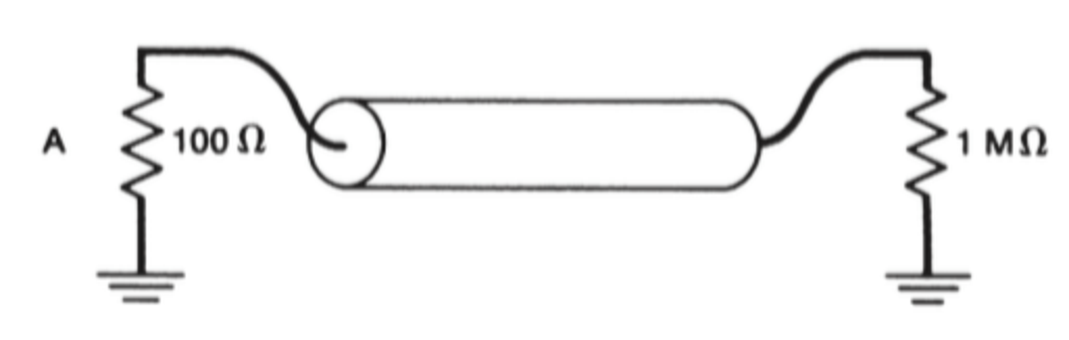
\includegraphics[width=.45\textwidth]{img/setup_A.pdf} \label{fig:term_a_setup}}
\hfill
 \subfloat[Termination A schematic]  {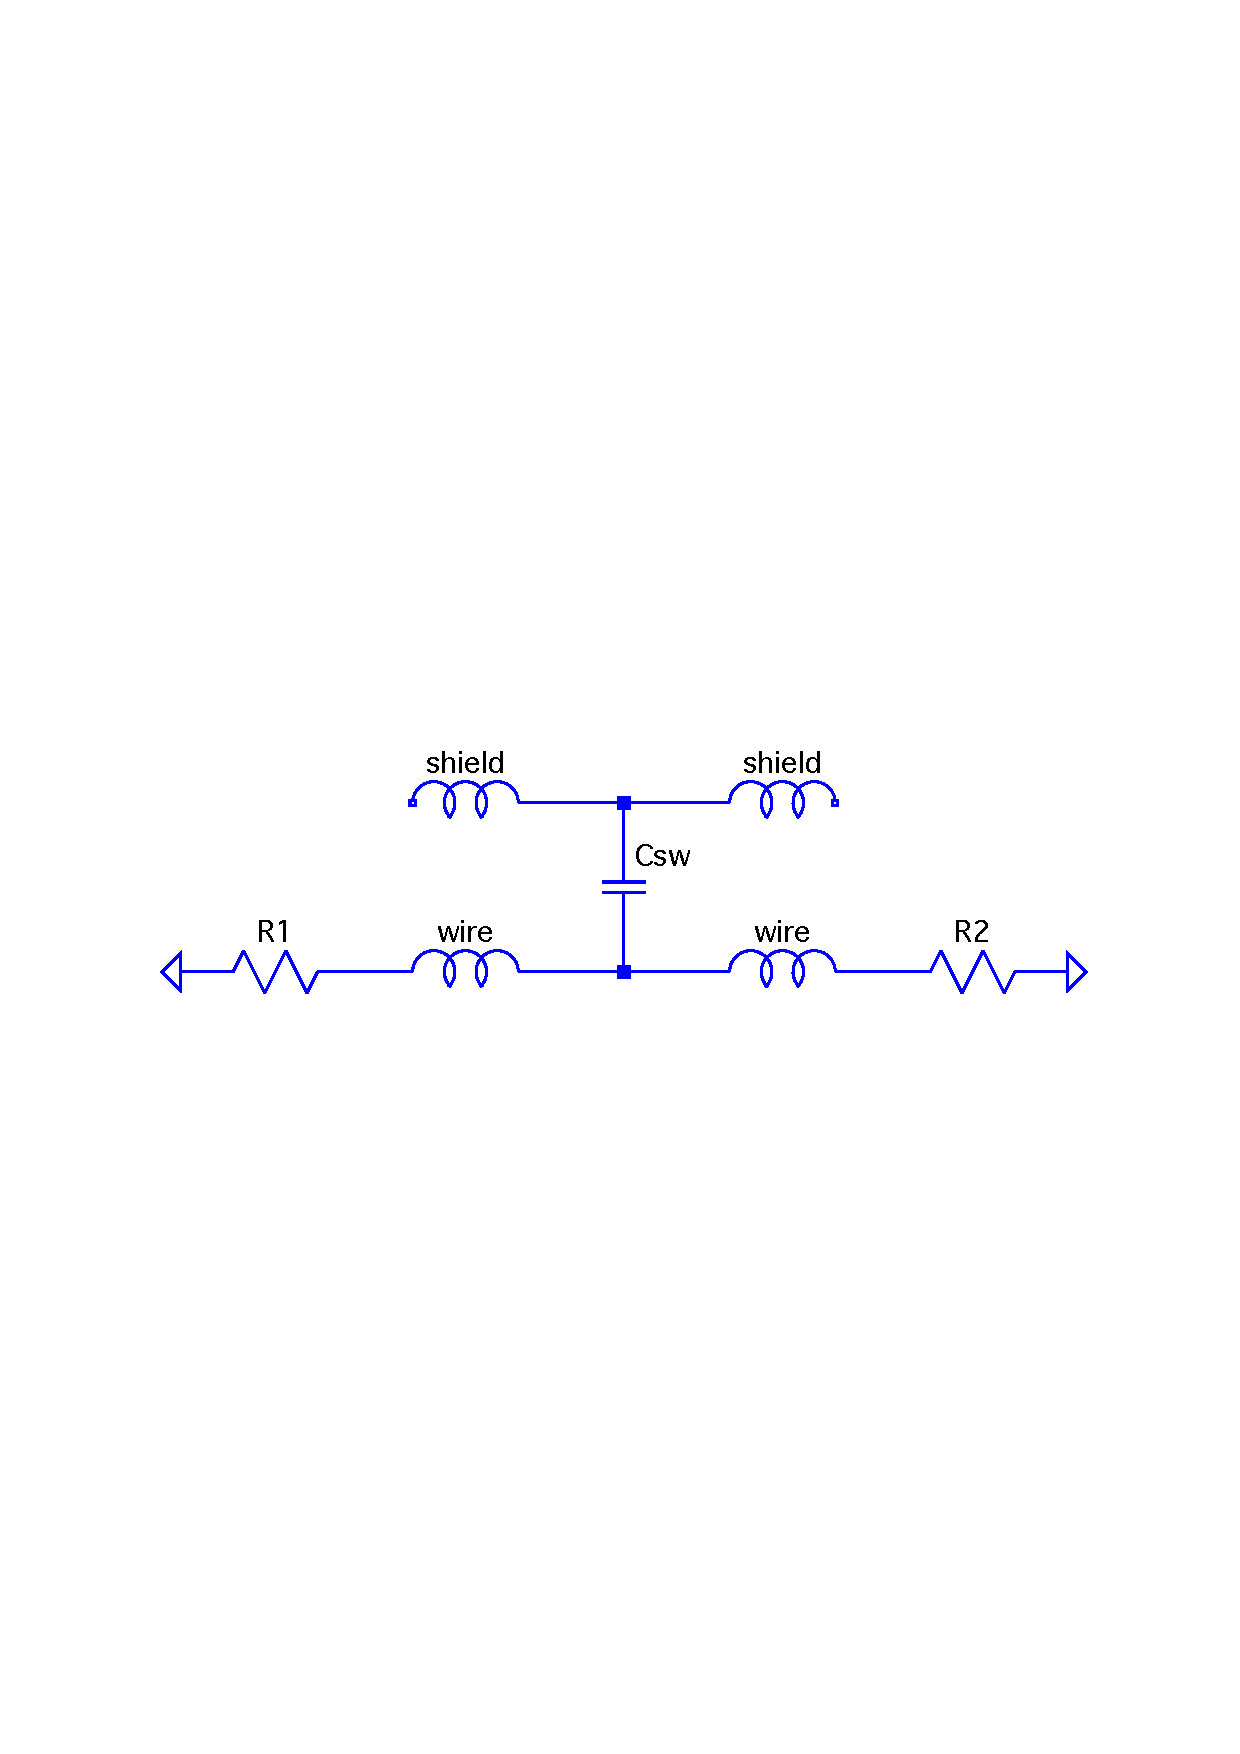
\includegraphics[width=.54\textwidth]{img/sch_A.pdf}\label{fig:term_a_sch}}
 \caption{Termination A setup and schematic} 
\label{fig:term_a} 
\end{figure}

\subsection{Termination B}
\begin{figure} [H]
  \centering 
  \subfloat[Termination B set up]  {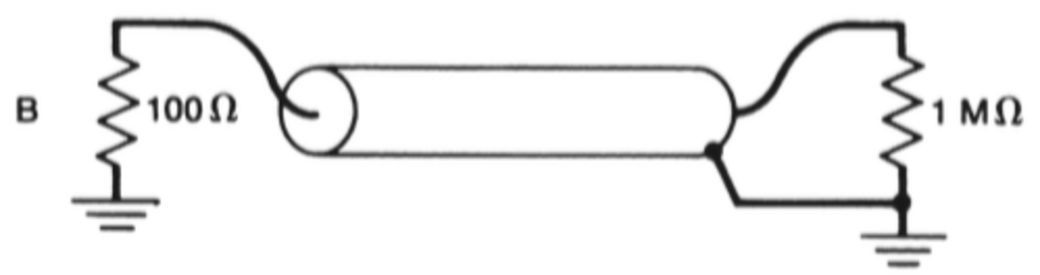
\includegraphics[width=.45\textwidth]{img/setup_B.pdf} \label{fig:term_b_setup}}
\hfill
 \subfloat[Termination B schematic]  {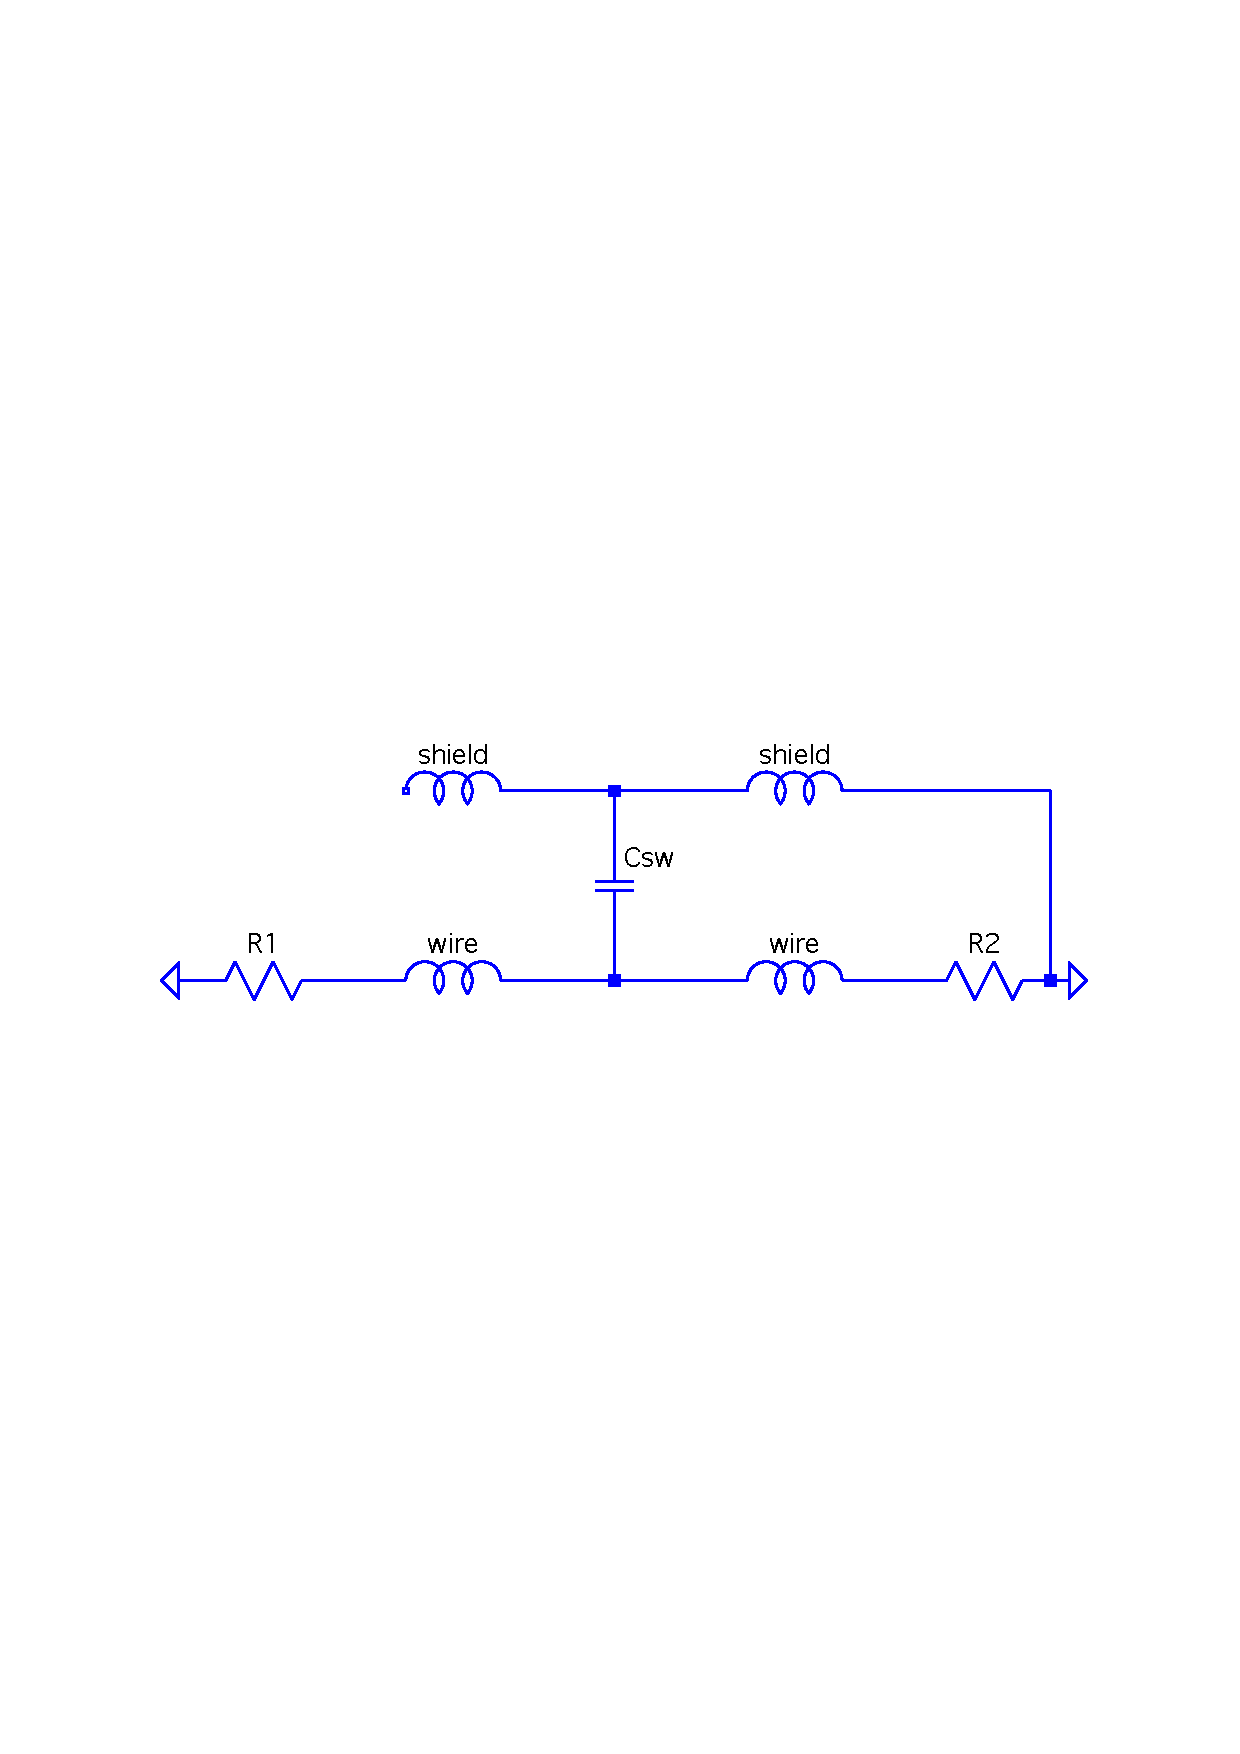
\includegraphics[width=.54\textwidth]{img/sch_B.pdf}\label{fig:term_b_sch}}
 \caption{Termination B setup and schematic} 
\label{fig:term_b} 
\end{figure}

\subsection{Termination C}
\begin{figure} [H]
  \centering 
  \subfloat[Termination C set up]  {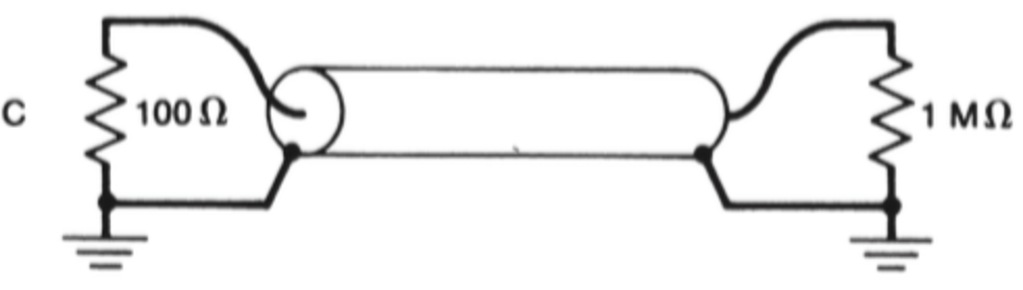
\includegraphics[width=.45\textwidth]{img/setup_C.pdf} \label{fig:term_c_setup}}
\hfill
 \subfloat[Termination C schematic]  {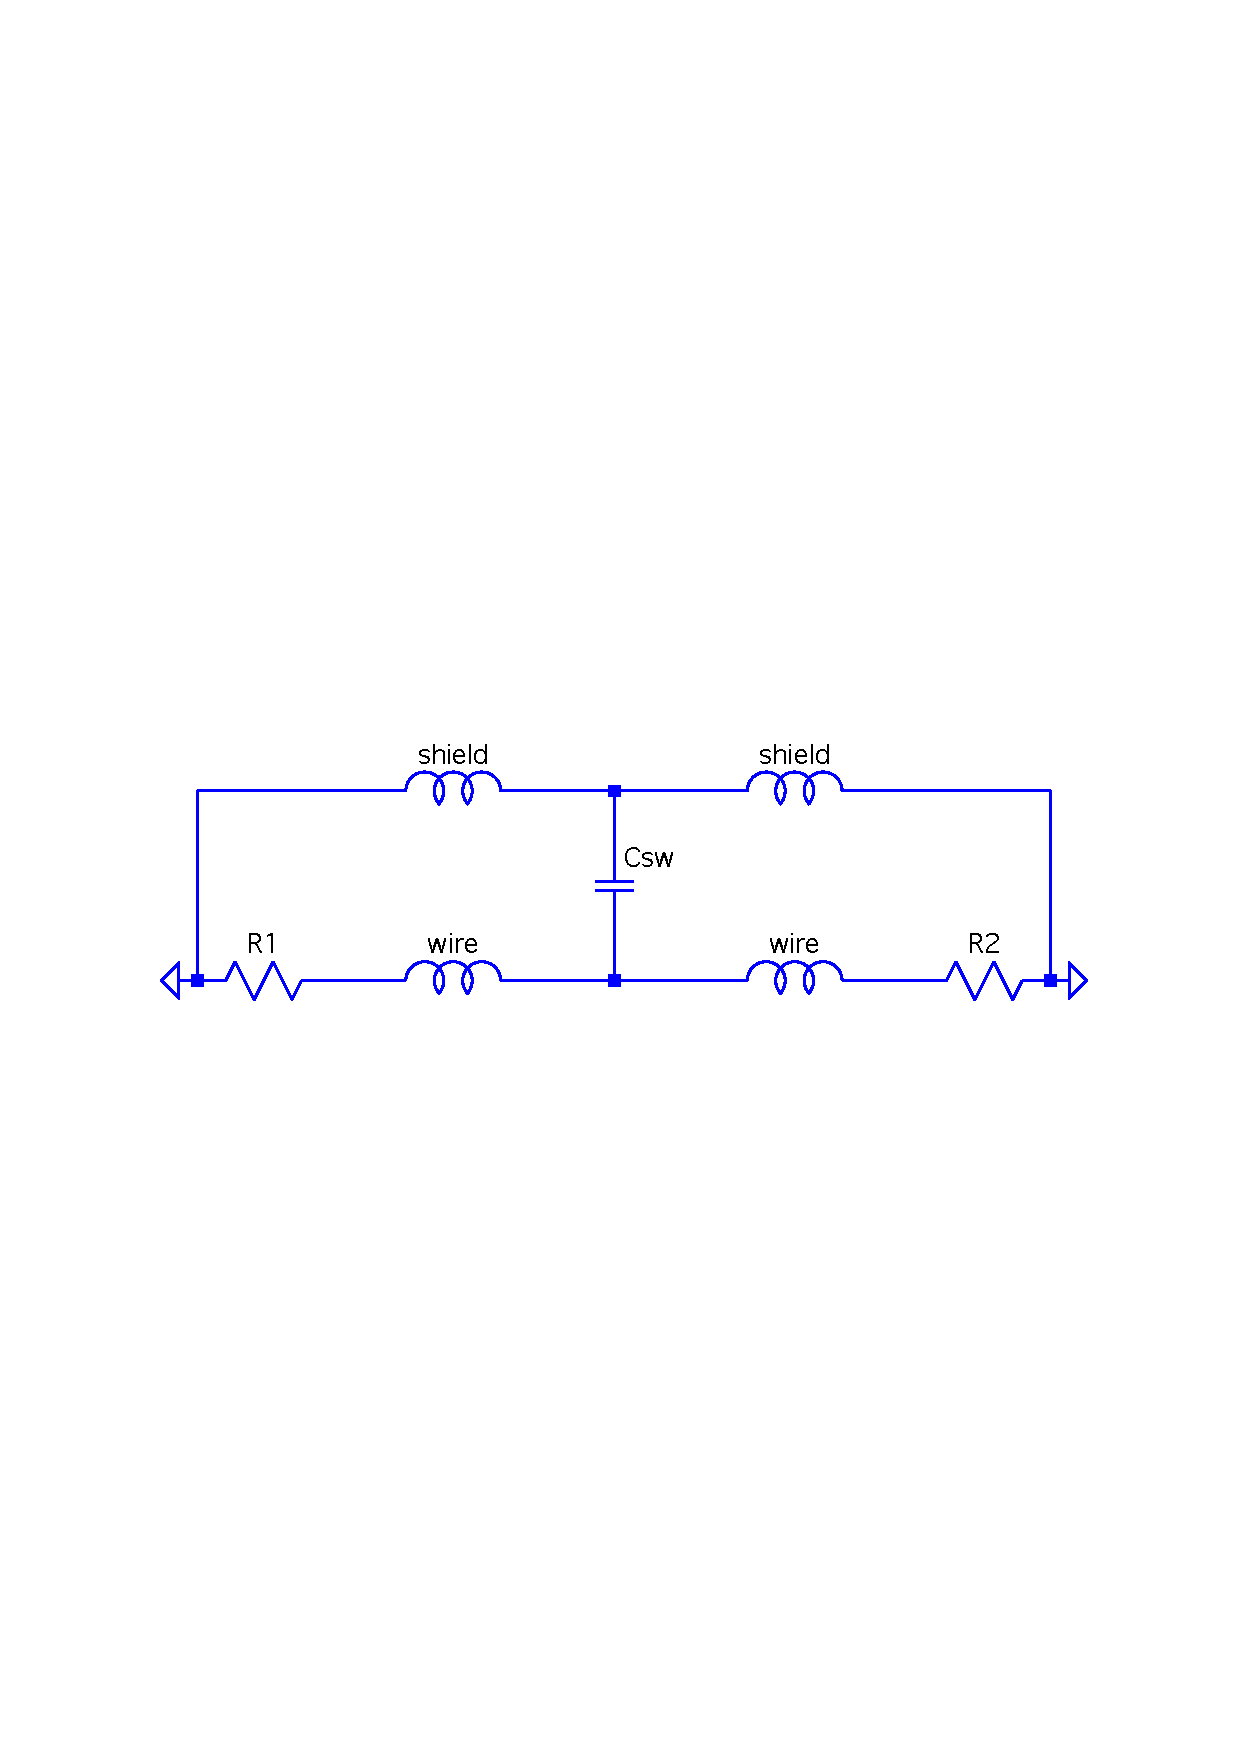
\includegraphics[width=.54\textwidth]{img/sch_C.pdf}\label{fig:term_c_sch}}
 \caption{Termination C setup and schematic} 
\label{fig:term_c} 
\end{figure}

\subsection{Termination D}
\begin{figure} [H]
  \centering 
  \subfloat[Termination D set up]  {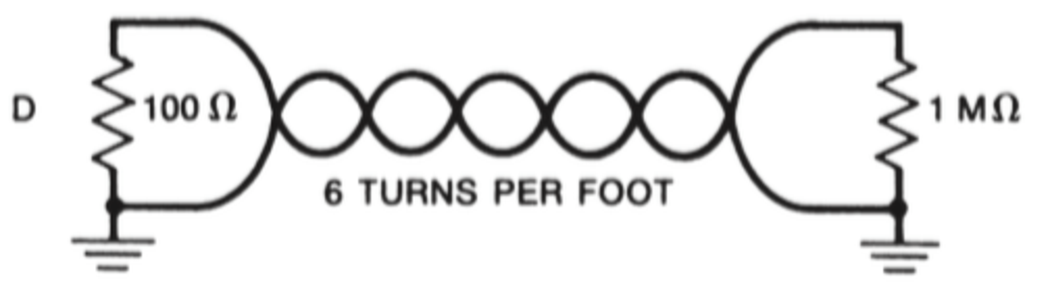
\includegraphics[width=.45\textwidth]{img/setup_D.pdf} \label{fig:term_d_setup}}
\hfill
 \subfloat[Termination D schematic]  {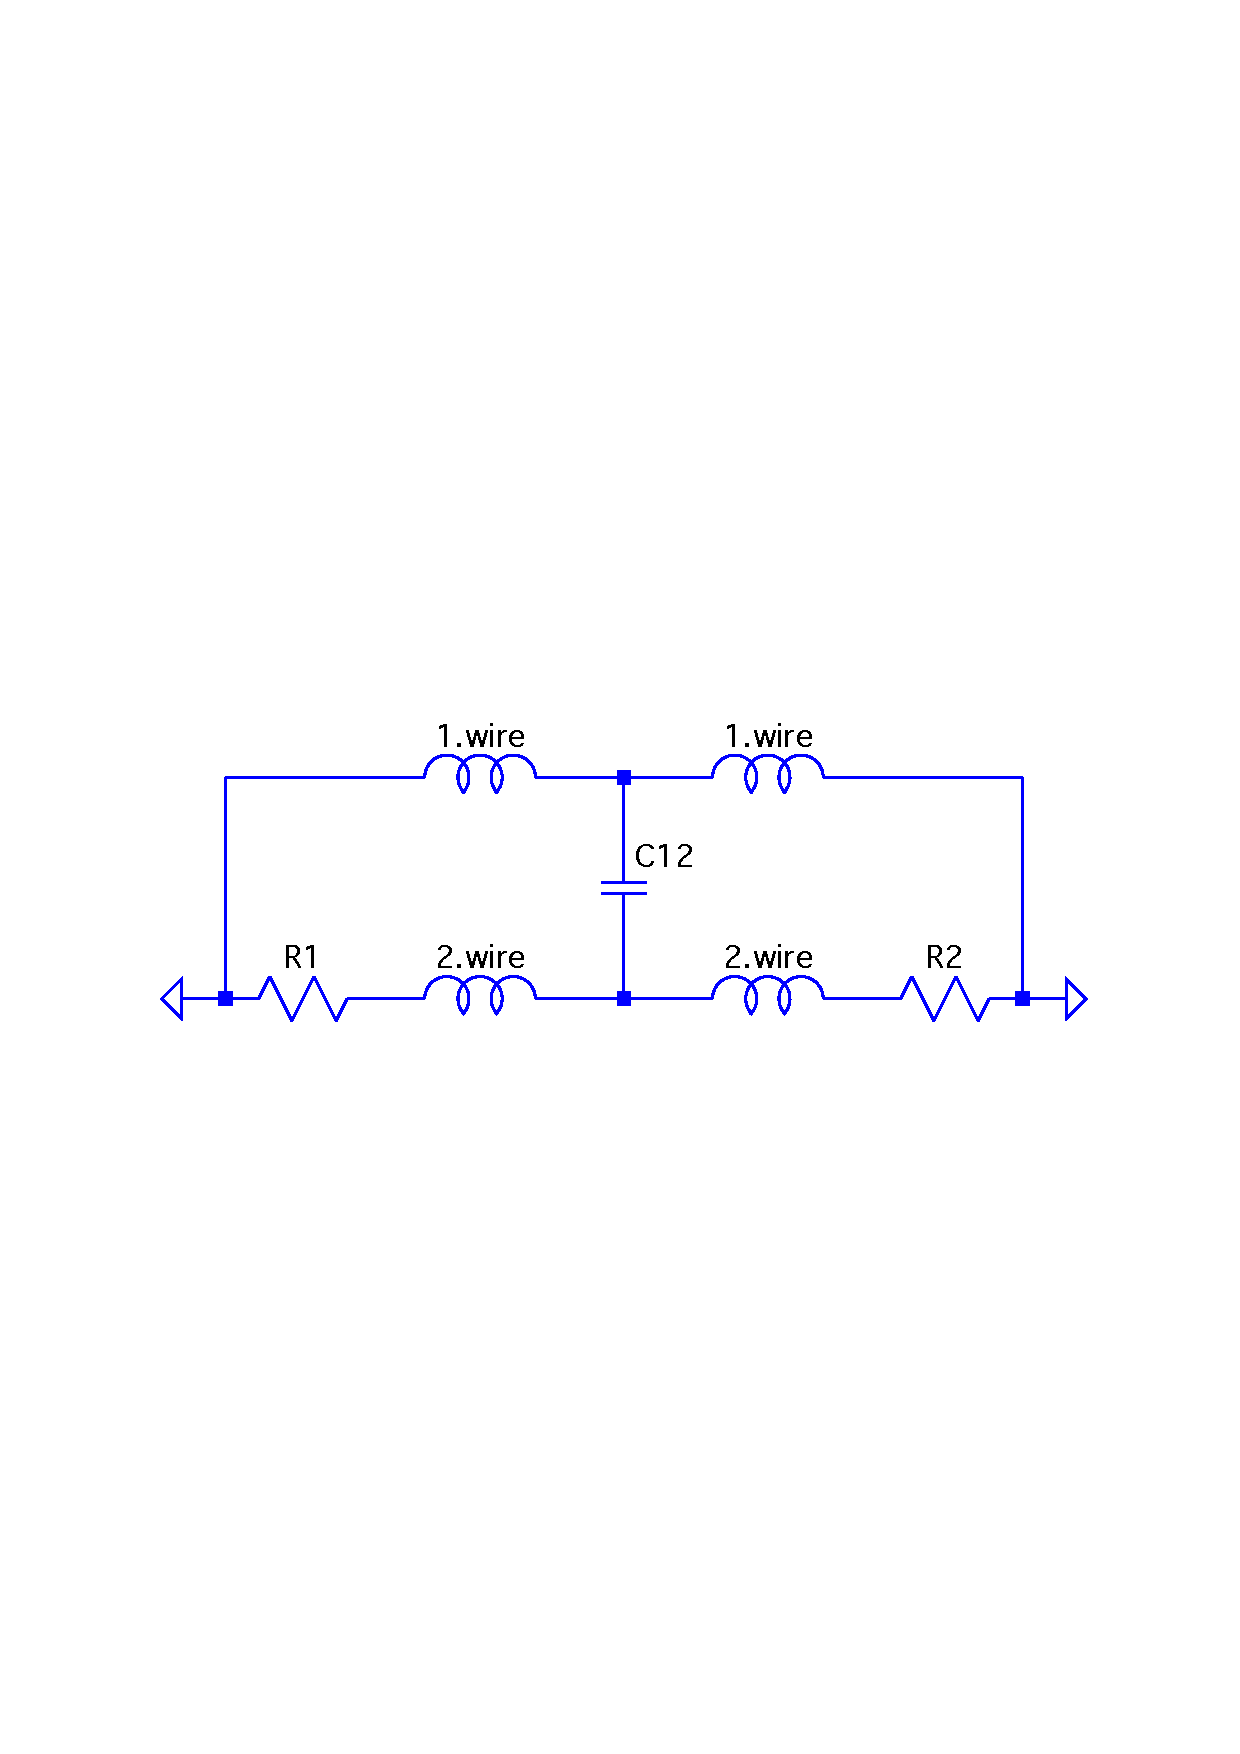
\includegraphics[width=.54\textwidth]{img/sch_D.pdf}\label{fig:term_d_sch}}
 \caption{Termination D setup and schematic} 
\label{fig:term_d} 
\end{figure}

\subsection{Termination E}
\begin{figure} [H]
  \centering 
  \subfloat[Termination E set up]  {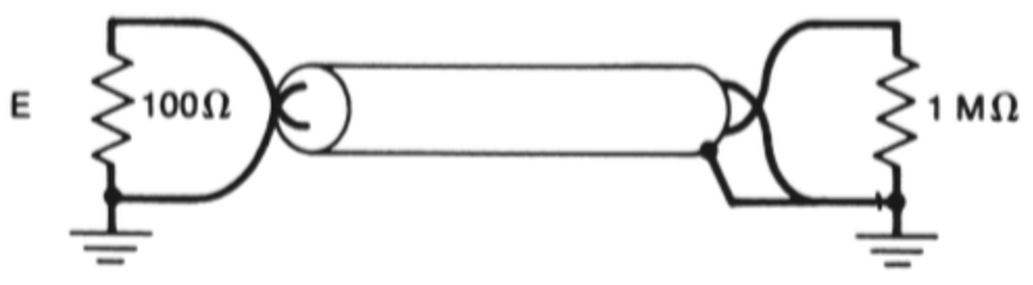
\includegraphics[width=.45\textwidth]{img/setup_E.pdf} \label{fig:term_e_setup}}
\hfill
 \subfloat[Termination E schematic]  {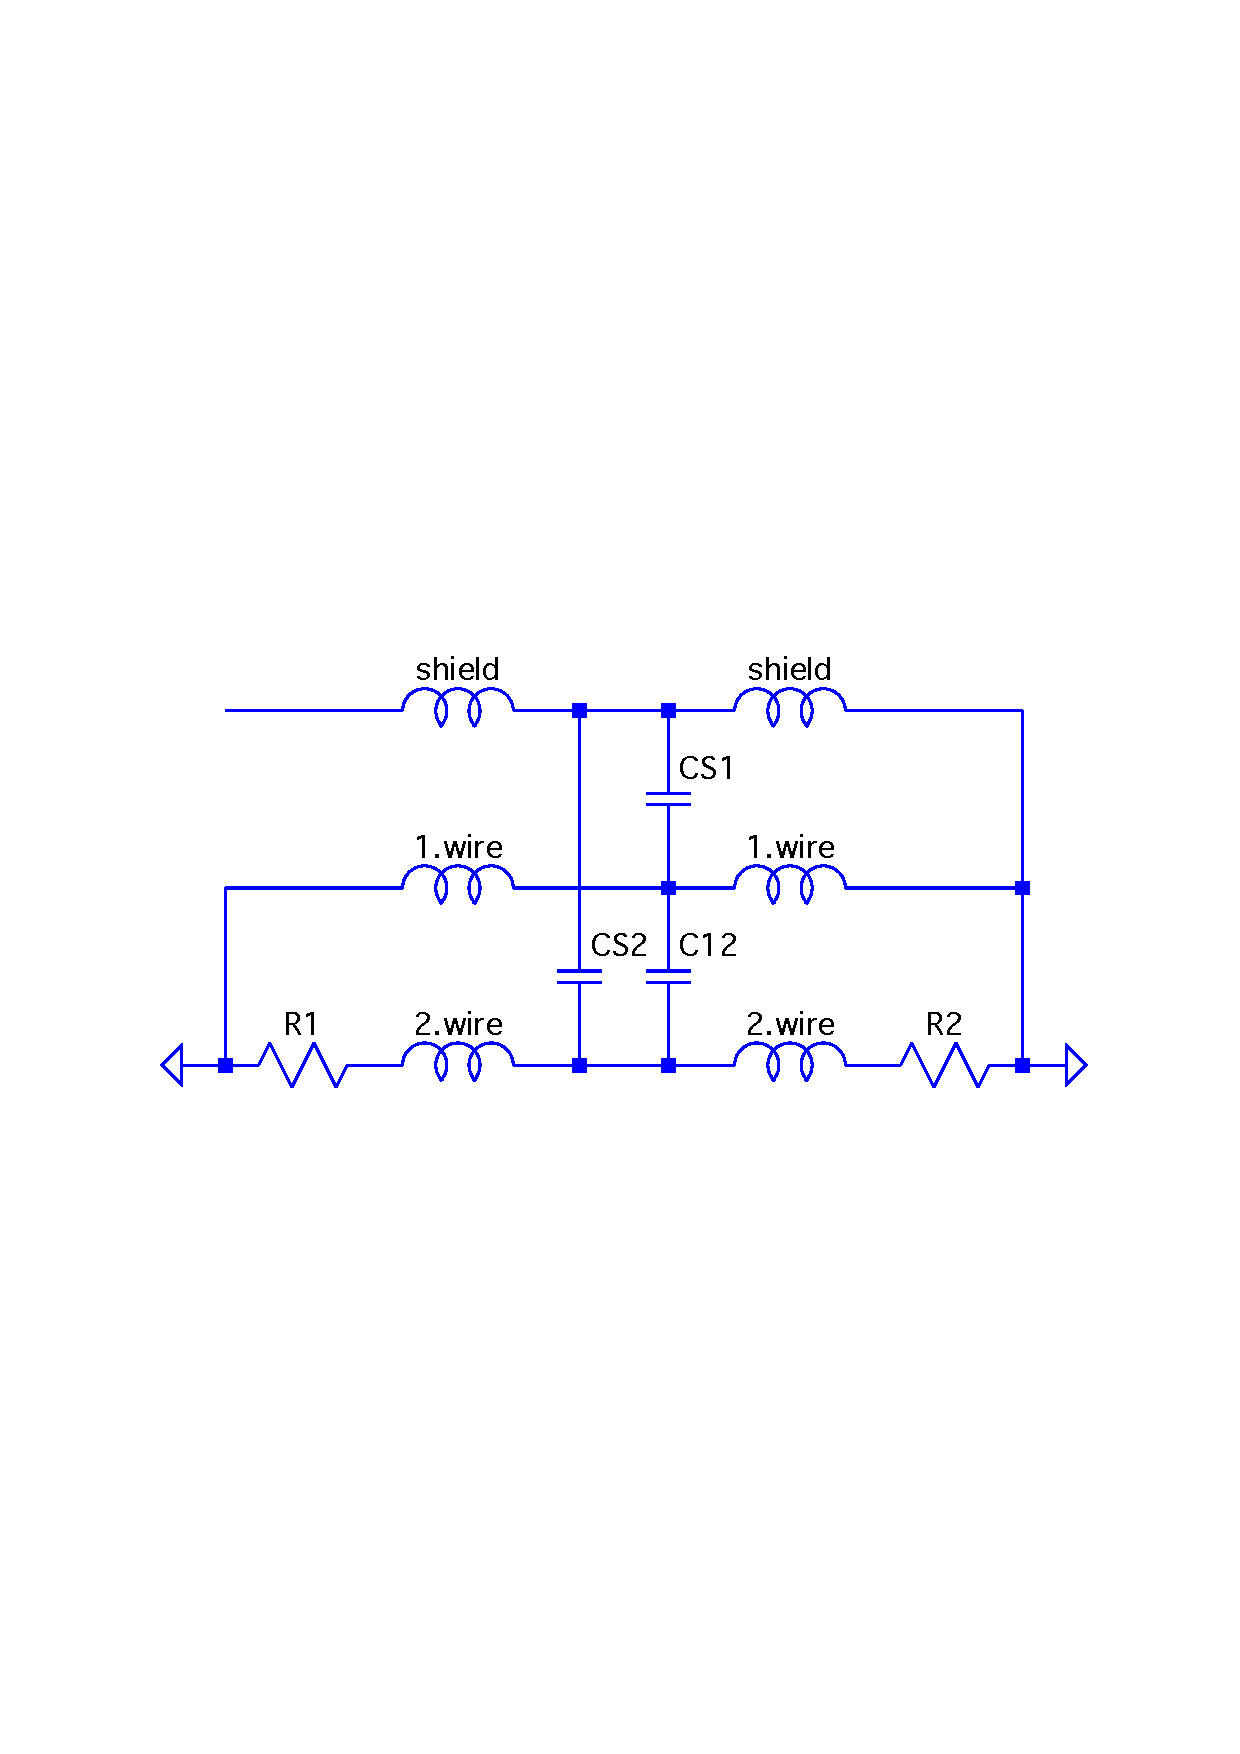
\includegraphics[width=.54\textwidth]{img/sch_E.pdf}\label{fig:term_e_sch}}
 \caption{Termination E setup and schematic} 
\label{fig:term_e} 
\end{figure}

\subsection{Termination F}
\begin{figure} [H]
  \centering 
  \subfloat[Termination F set up]  {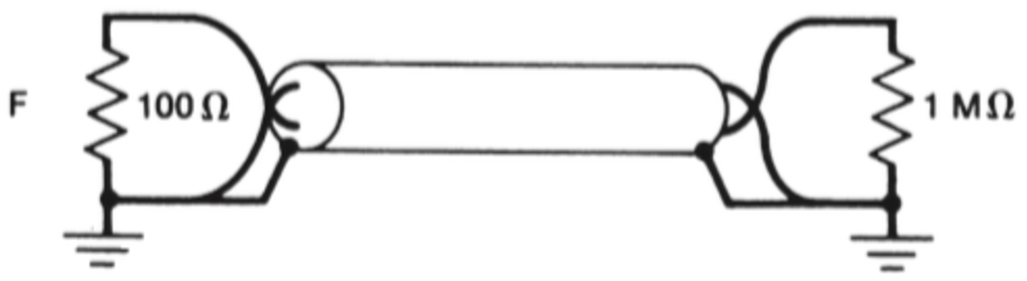
\includegraphics[width=.45\textwidth]{img/setup_F.pdf} \label{fig:term_f_setup}}
\hfill
 \subfloat[Termination F schematic]  {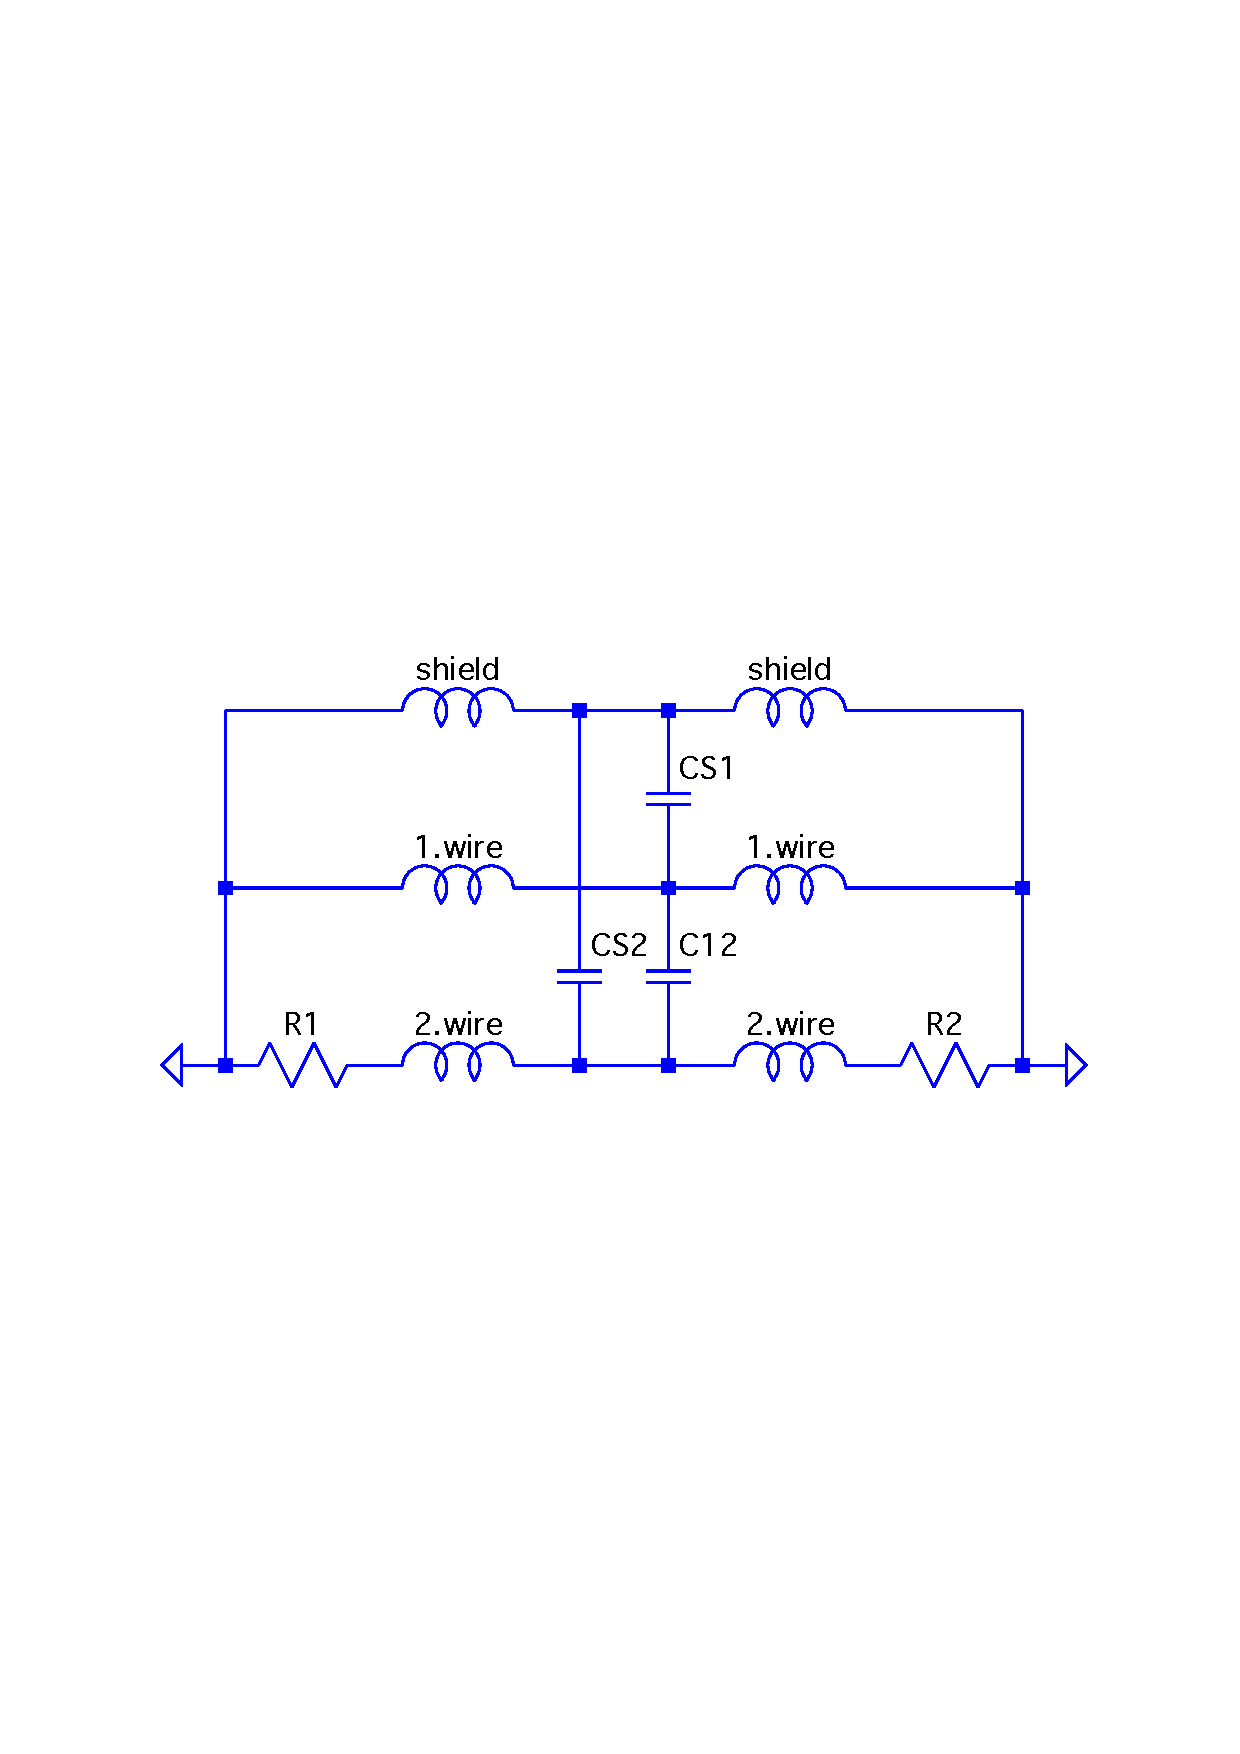
\includegraphics[width=.54\textwidth]{img/sch_F.pdf}\label{fig:term_f_sch}}
 \caption{Termination F setup and schematic} 
\label{fig:term_f} 
\end{figure}

\subsection{Termination G}
\begin{figure} [H]
  \centering 
  \subfloat[Termination G set up]  {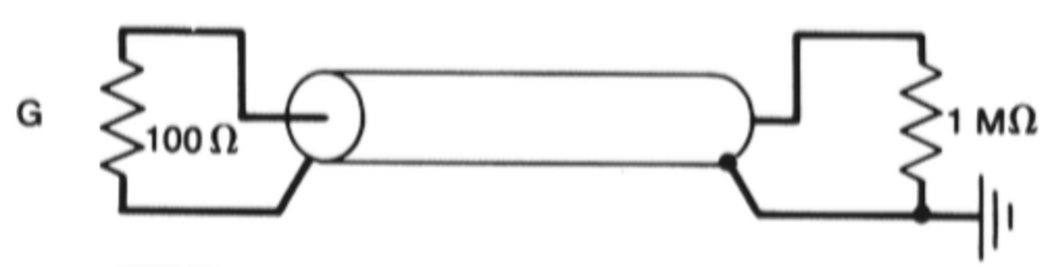
\includegraphics[width=.45\textwidth]{img/setup_G.pdf} \label{fig:term_g_setup}}
\hfill
 \subfloat[Termination G schematic]  {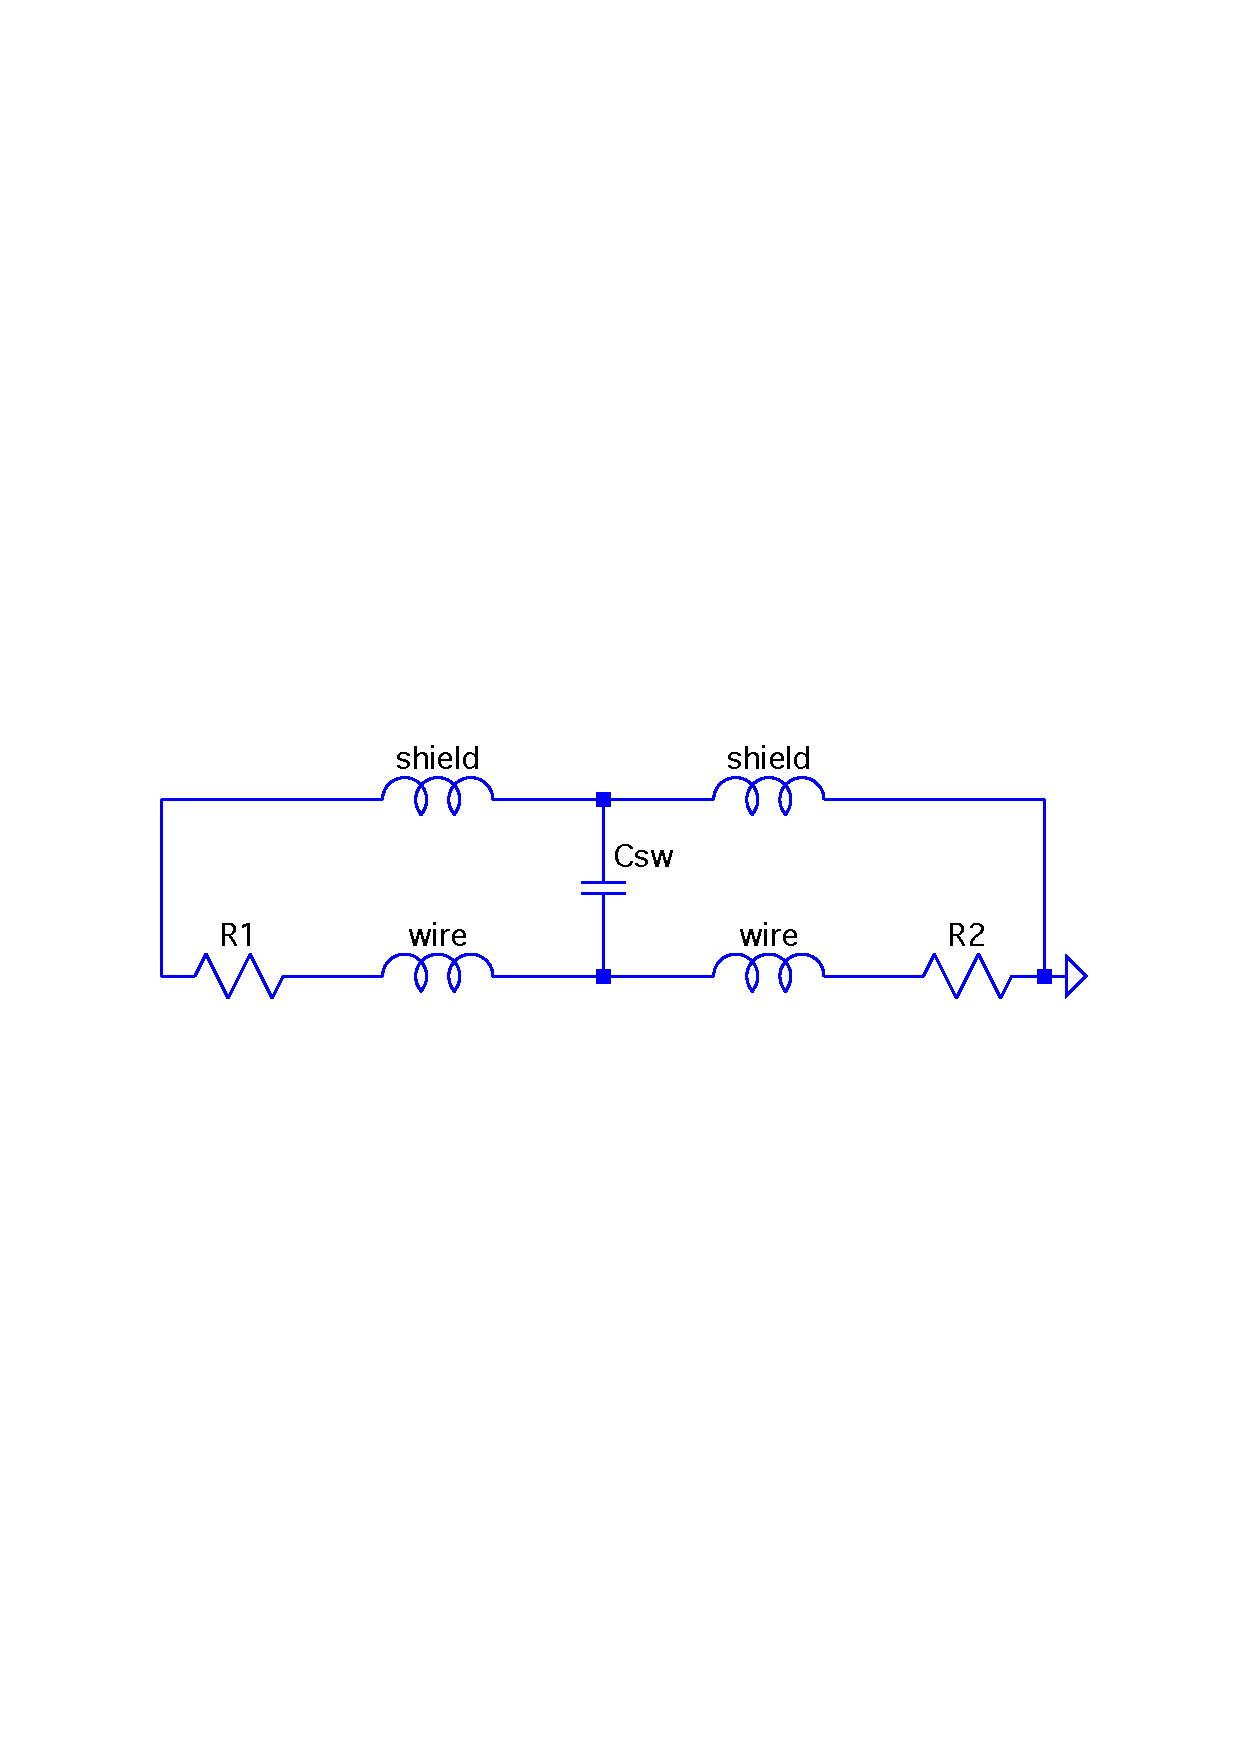
\includegraphics[width=.54\textwidth]{img/sch_G.pdf}\label{fig:term_g_sch}}
 \caption{Termination G setup and schematic} 
\label{fig:term_g} 
\end{figure}

\subsection{Termination H}
\begin{figure} [H]
  \centering 
  \subfloat[Termination H set up]  {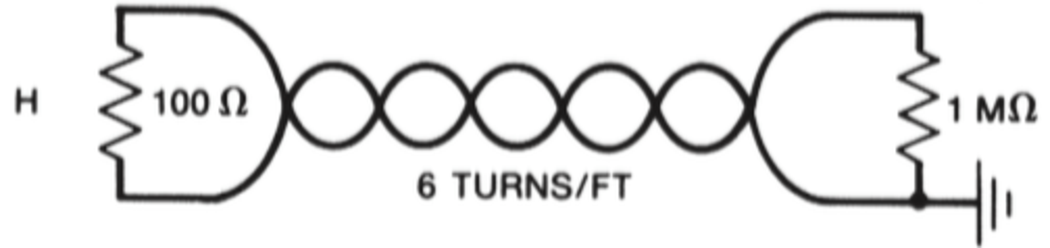
\includegraphics[width=.45\textwidth]{img/setup_H.pdf} \label{fig:term_h_setup}}
\hfill
 \subfloat[Termination H schematic]  {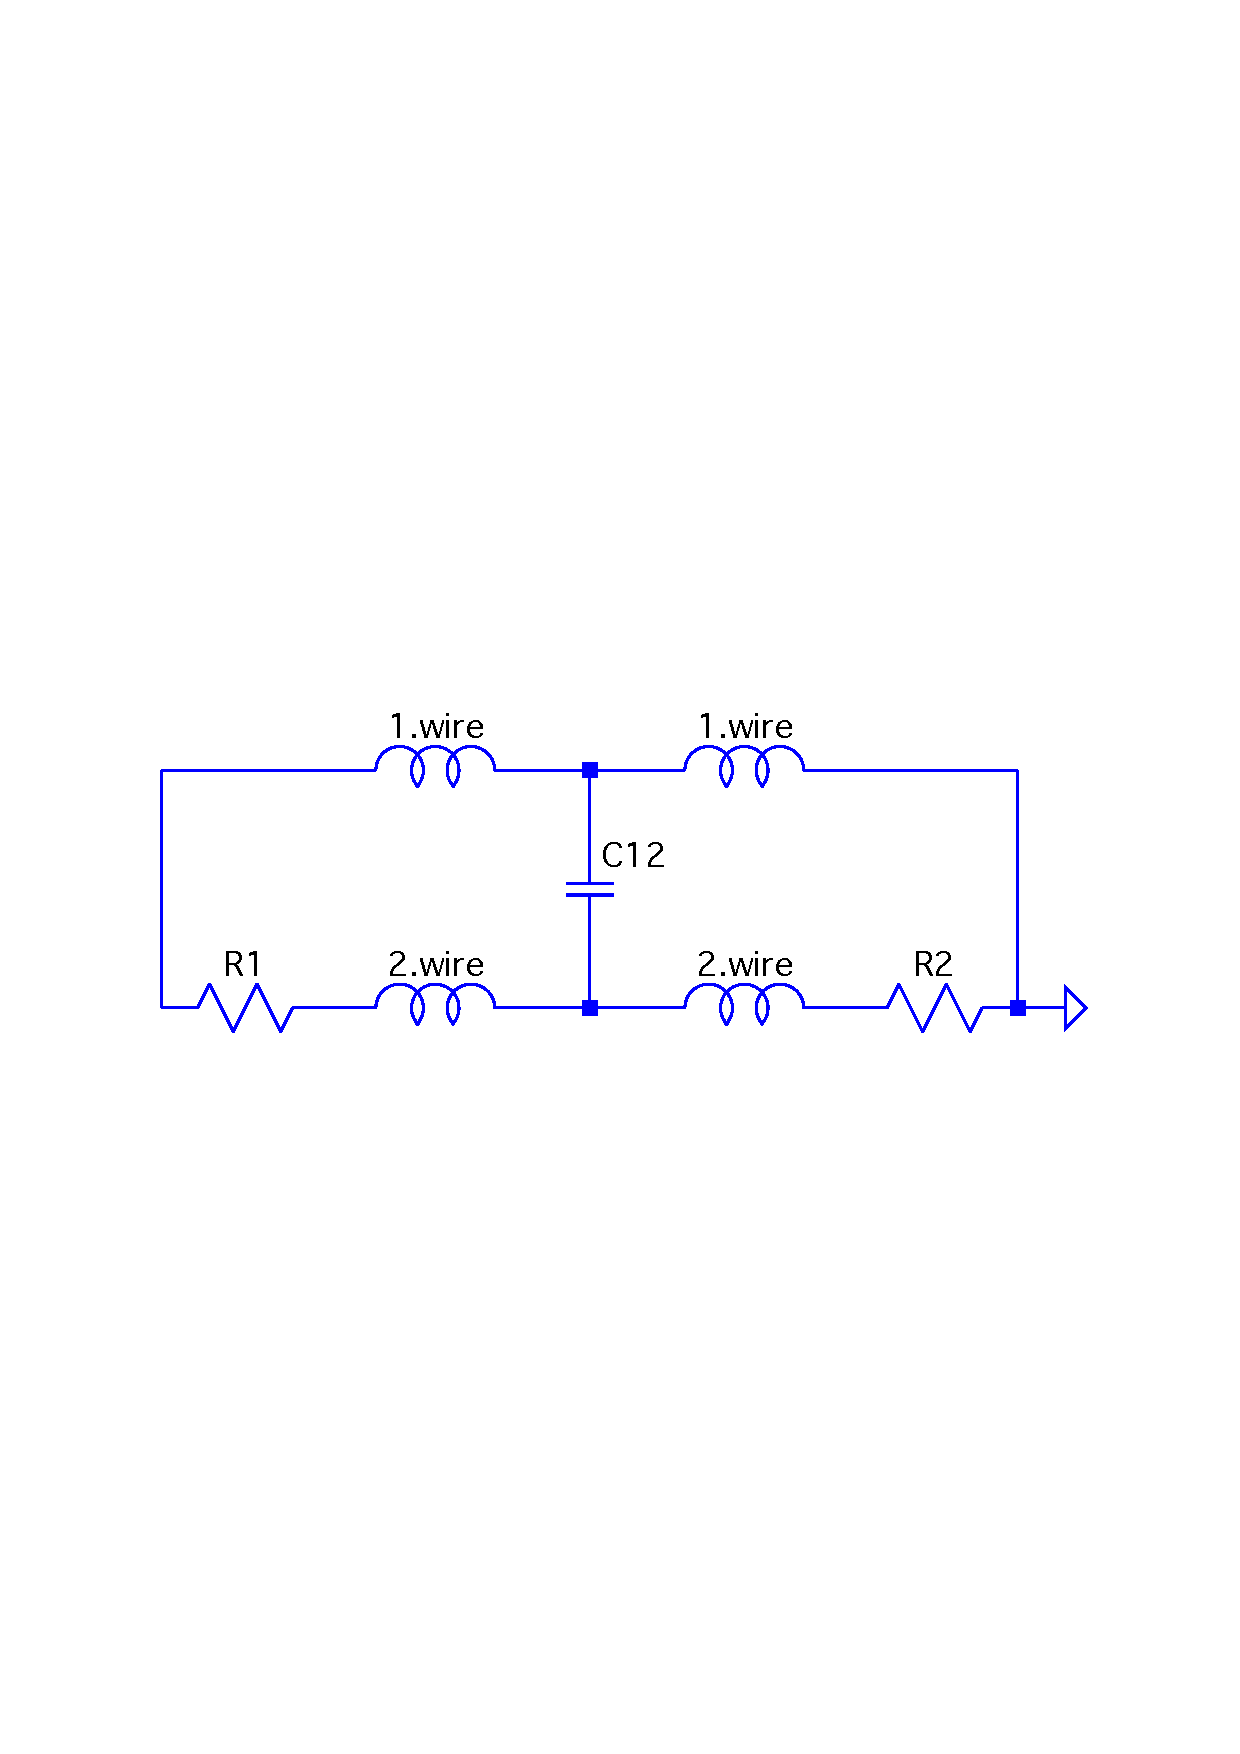
\includegraphics[width=.54\textwidth]{img/sch_H.pdf}\label{fig:term_h_sch}}
 \caption{Termination H setup and schematic} 
\label{fig:term_h} 
\end{figure}

\subsection{Termination I}
\begin{figure} [H]
  \centering 
  \subfloat[Termination I set up]  {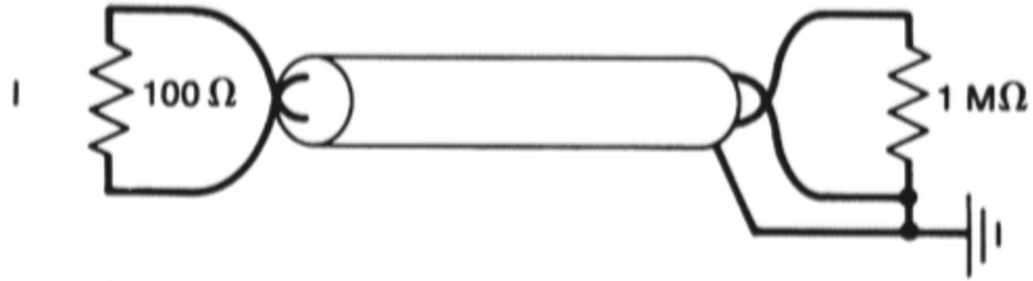
\includegraphics[width=.45\textwidth]{img/setup_I.pdf} \label{fig:term_i_setup}}
\hfill
 \subfloat[Termination I schematic]  {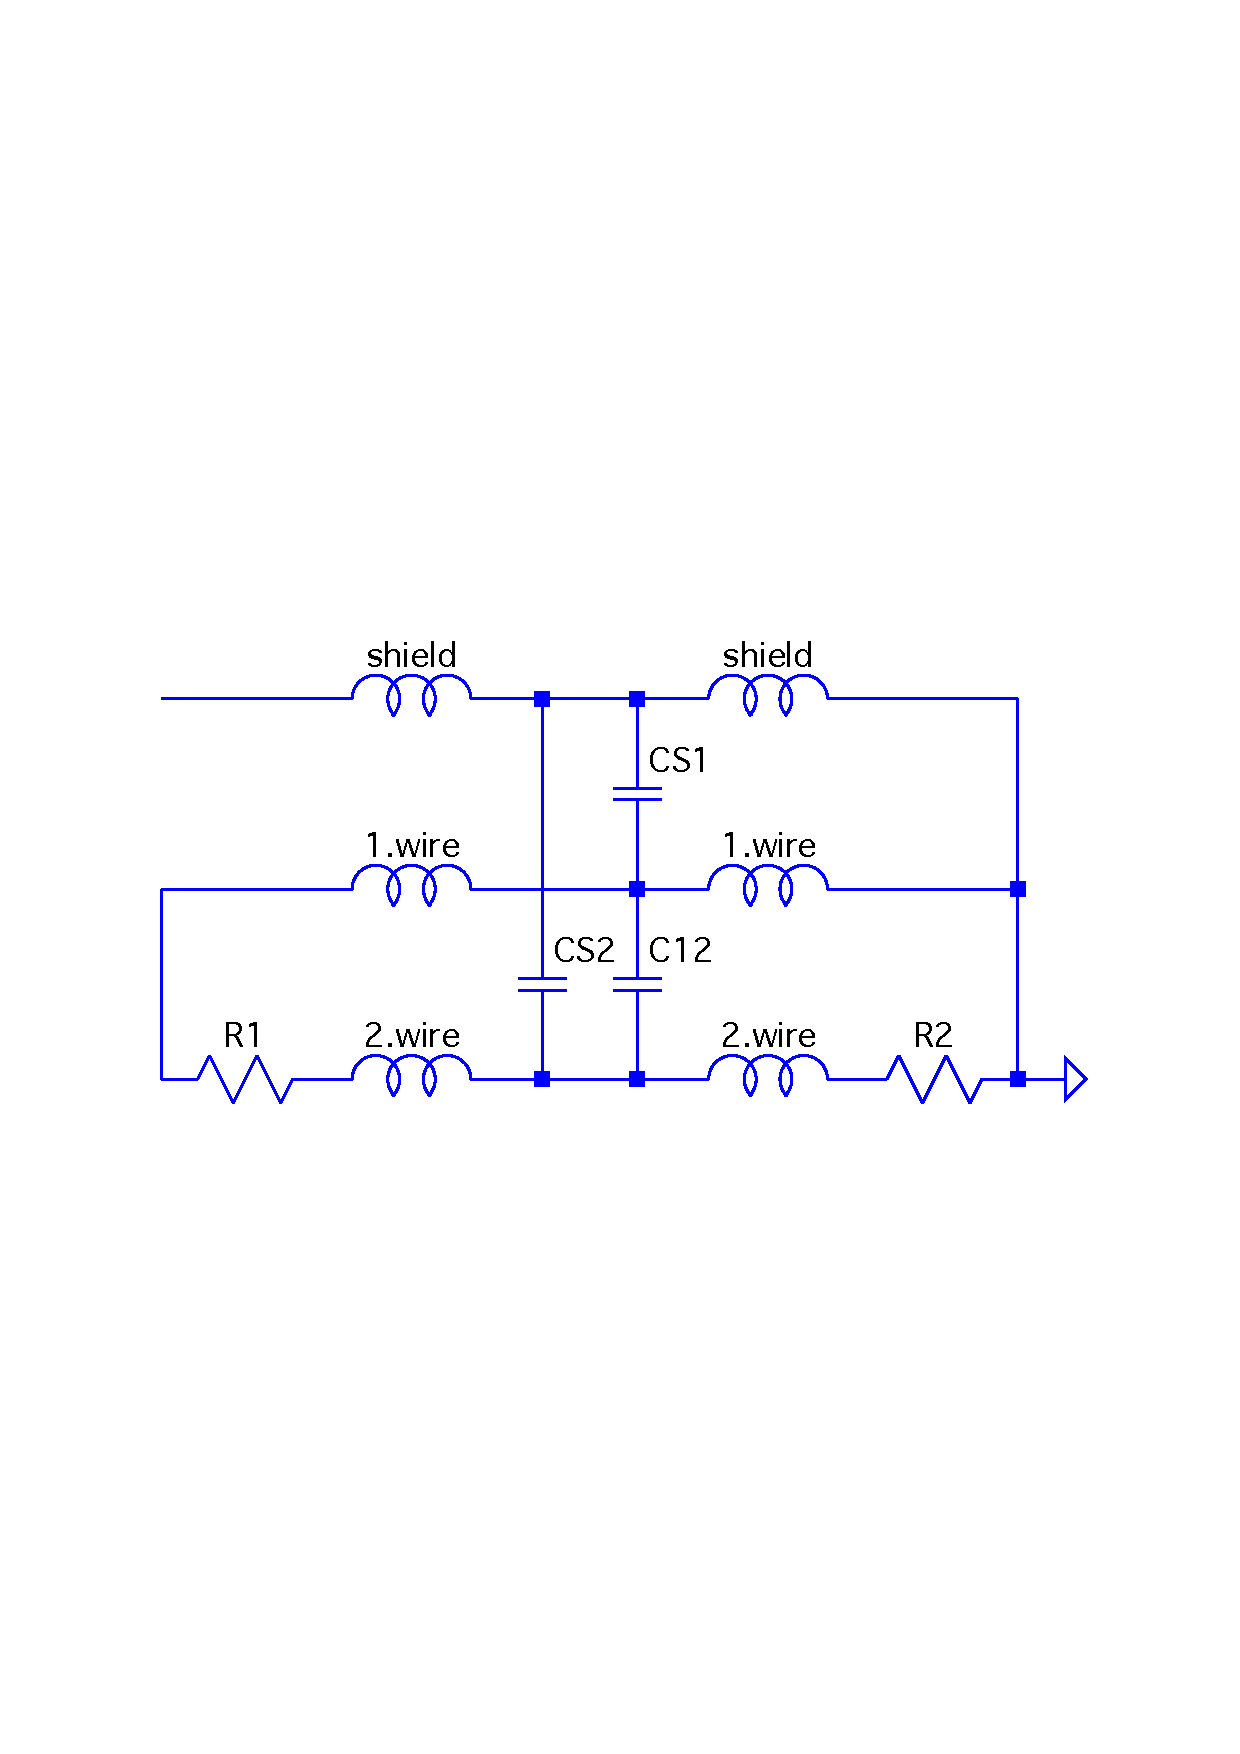
\includegraphics[width=.54\textwidth]{img/sch_I.pdf}\label{fig:term_i_sch}}
 \caption{Termination I setup and schematic} 
\label{fig:term_i} 
\end{figure}

\subsection{Termination J}
\begin{figure} [H]
  \centering 
  \subfloat[Termination J set up]  {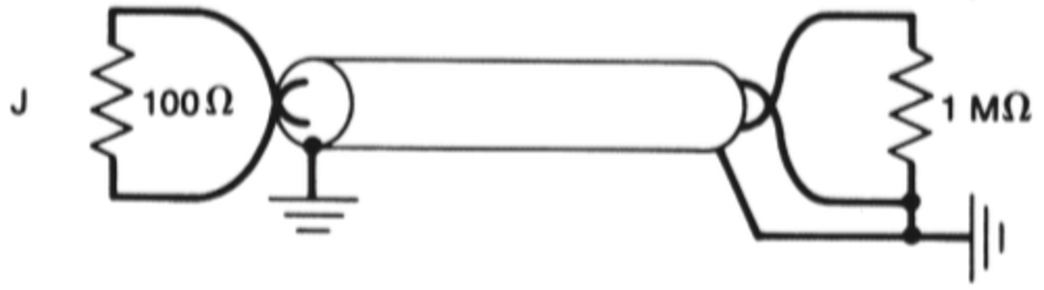
\includegraphics[width=.45\textwidth]{img/setup_J.pdf} \label{fig:term_j_setup}}
\hfill
 \subfloat[Termination J schematic]  {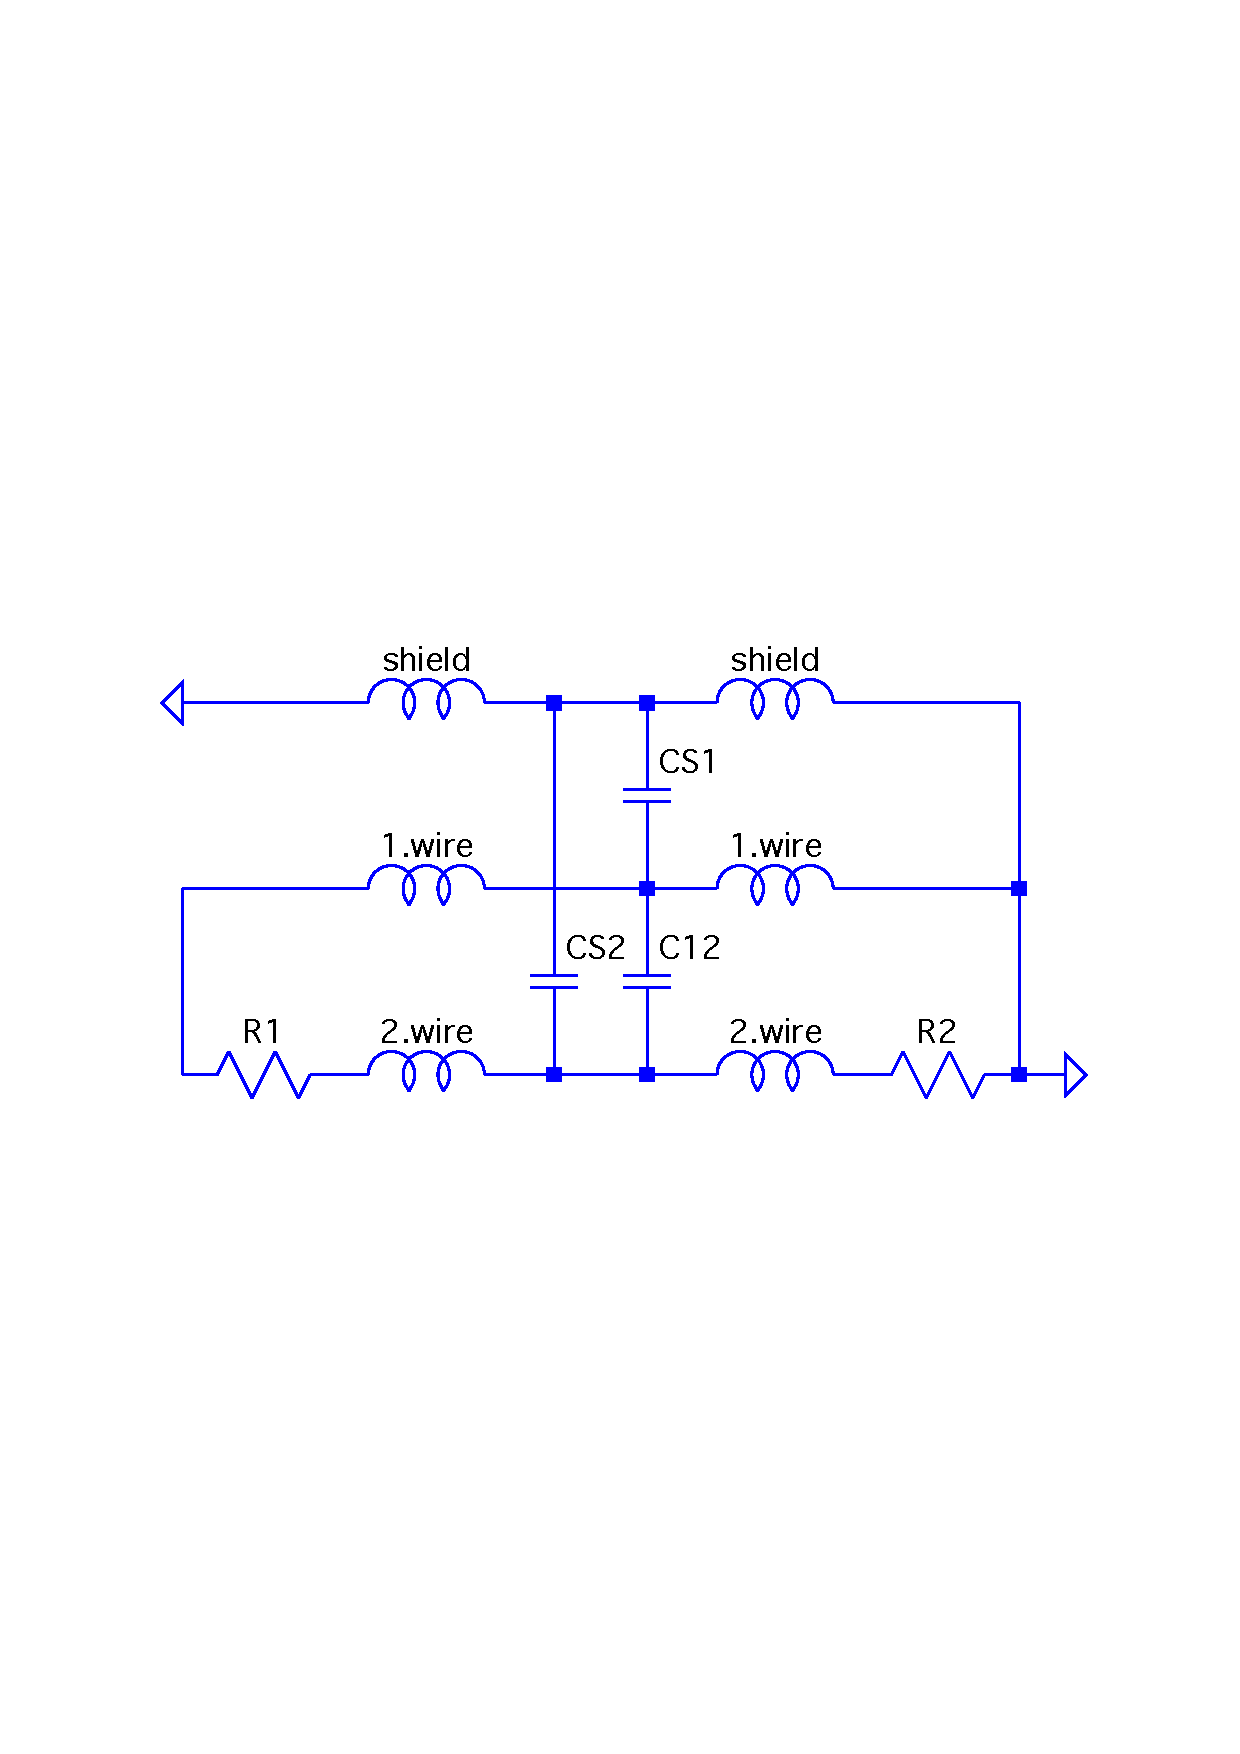
\includegraphics[width=.54\textwidth]{img/sch_J.pdf}\label{fig:term_j_sch}}
 \caption{Termination J setup and schematic} 
\label{fig:term_j} 
\end{figure}

\subsection{Termination K}
\begin{figure} [H]
  \centering 
  \subfloat[Termination K set up]  {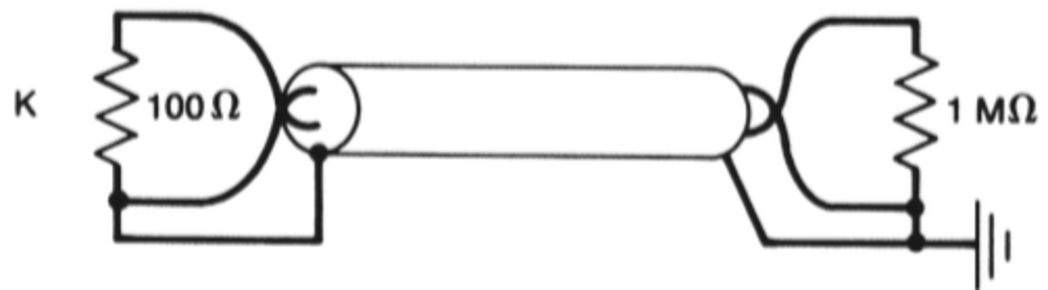
\includegraphics[width=.45\textwidth]{img/setup_K.pdf} \label{fig:term_k_setup}}
\hfill
 \subfloat[Termination K schematic]  {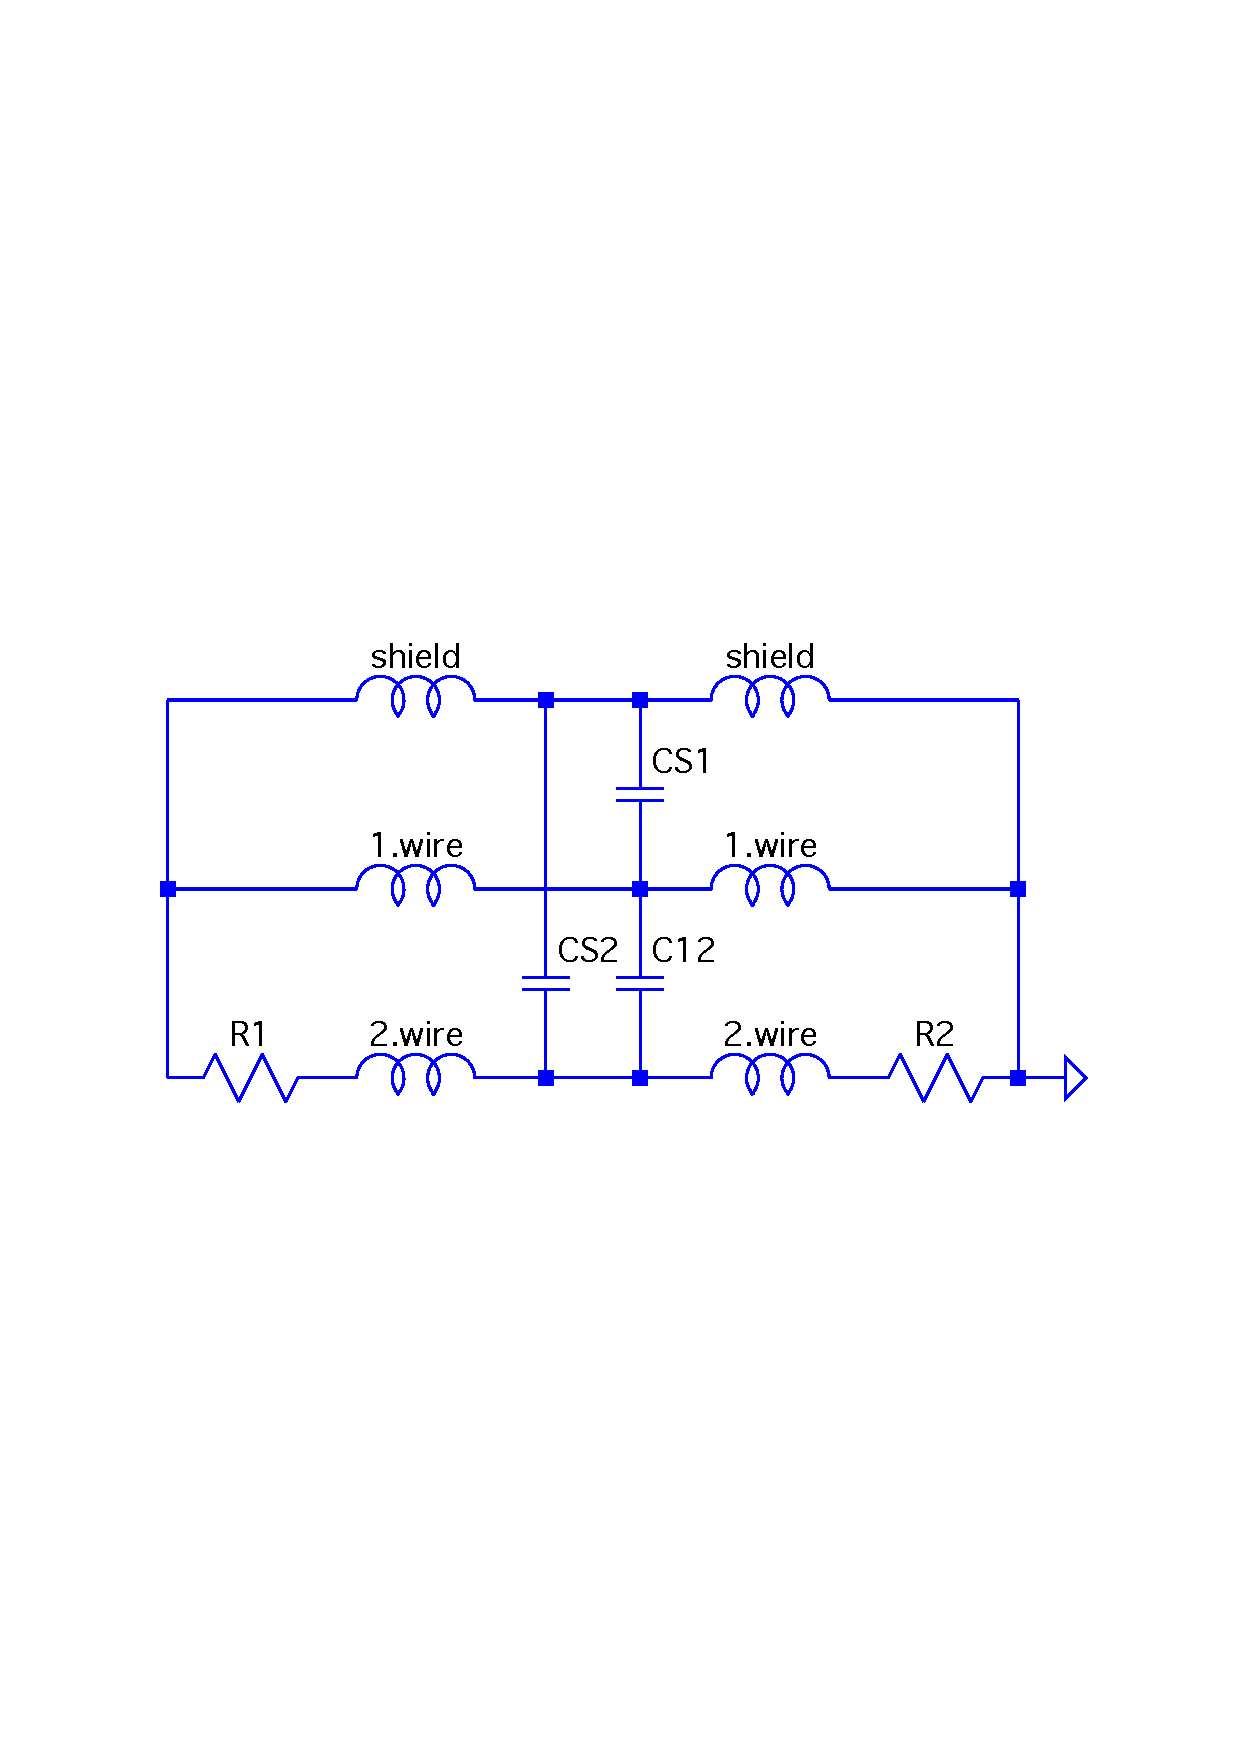
\includegraphics[width=.54\textwidth]{img/sch_K.pdf}\label{fig:term_k_sch}}
 \caption{Termination K setup and schematic} 
\label{fig:term_k} 
\end{figure}

%% TASK 2
\section{In this experiment, we use a lot the decibel scale. $VdB = 20log \big(\frac{Vpp}{\sqrt{2}}\big)$. \\
What describes the greatest change: Going from -21 to -23 dB, or to go from -72 to -78dB? (Calculate and explain).}
-21 and -23 dB correspond to 0.12604 and 0.10012 $V_{rms}$. The difference is 0.02592. \\
Similarly -72 and -78 dB correspond 0.00036 to and 0.00018 $V_{rms}$. The difference is 0.00018. \\
This means -21 to -23 dB is the greatest change in dB scale.

%% TASK3
\section{Use termination card A together with all cables. Write down the results}
For this task, primary coil P2 was chosen. Input to the primary was sinusoidal signal of frequency 50 kHz and amplitude 10 Vpp. The oscilloscope sampling frequency was 400 kS/sec. Observed signal strenght with termination A connected to various cables are as follow in figure \ref{fig:task3} .
\begin{figure} [H] %% table as picx
  \centering 
  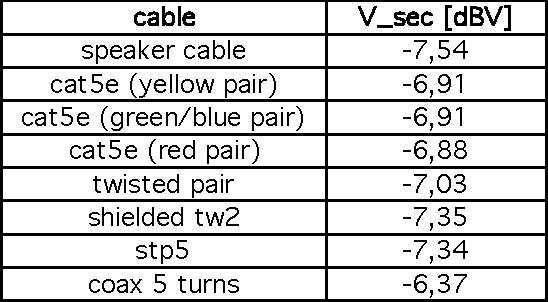
\includegraphics[width=0.5\textwidth]{img/task3_data.pdf} 
  \caption{Termination A with all cables}
  \label{fig:task3} 
\end{figure}

\subsection{Does shielding have something to say with this assignment? Explain}
From the above observation, we can say that shielding has no effect on noise signal through various cable type. It is because only the to end of the circuit is grounded and shield is completely floating. 

\subsection{What factors are causing the results to be not exactly identical for the cables? Explain your answer.}
There may be various factors but most important is the cable type. For example TP cancels the magnetic field around it which can clearly be seen in the above table.

%% TASK4
\section{Use termination card A with one of the cables.}
Coaxial cable with 5 turn was chosen as secondary coil. 
\subsection{Place a sheet of aluminium foil under the coils. How does this affect the result? Explain.}
While placing the aluminium foil under the coils, the signal in the secondary coil was reduced to -16.8 dB which is significant reduction when we compare with -6.37 dB obtained in task 3. It looks like aluminium foil with large surface area is observing more magnetic fields resulting in less magnetic fields on secondary coil. 

\subsection{On the bench there is probably other objects that may affect the results, and to some extent can bench itself affect the result. Try to move around a bit on the measurement configuration. Identify three objects or factors affecting measurement results, and explain how they affect.}
The observation results with random objects are as tabulated in figure \ref{fig:task4b}.
\begin{figure} [H] %% table as picx
  \centering 
  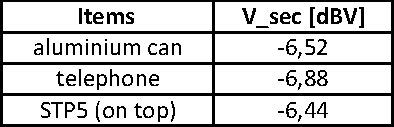
\includegraphics[width=0.5\textwidth]{img/task4b_data.pdf} 
  \caption{Random objects observation}
  \label{fig:task4b} 
\end{figure}
We did not observe much difference. But while placing a mobile set with flat surface covered with metal, the signal was slightly reduced. It should be the effect like that of aluminium foil above.

%%TASK 5
\section{Measure the signal strength of the 50kHz signal for terminals A-F. Record the results in a table.} 
For this task primary coil P2 and secondary coil STP was used. Sampling frequency of the oscilloscope was 400 kS/sec as earlier. The results are as follows. All the circuits in these terminations are grounded at both ends.
\begin{figure} [H] %% table as picx
  \centering 
  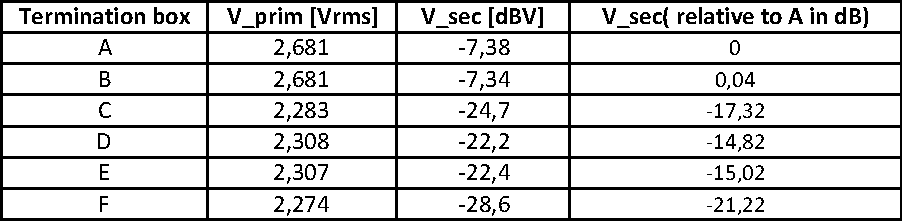
\includegraphics[width=0.9\textwidth]{img/task5_data.pdf} 
  \caption{Termination A-F observations}
  \label{fig:task5b} 
\end{figure}
\subsection{Is the inductive or capacitive noise that dominates for these terminations? Explain.}
It is inductive noise that dominates for these terminals. Because except in A and D, the shield is grounded in all other termination. And once the shield is grounded and if the shield is completely covering the receiver conductor, capacitive noise is mostly removed. However we can see in case of C and F terminations, there is some reduction in inductive coupling too.
\subsection{Describe how the terminals A-F acts in relation to each other and how the differences between them are involved.}
A: This termination neither shield inductive noise nor capacitative noise because both the ends of the shield are floating. \\
B: This termination shields capacitative noise but not inductive noise as the shield is grounded only at one end. \\
C: As both ends of the shield is grounded, it provides better shielding of inductive noise. But the shield loop area is larger due to both end grounding of the shield and hence some noise voltage is induced in the shield.\\
D: Twisted pair by itself cancels some magnetic fields but it has not shield and the low impedance ground loop area is large. so both inductive and capacitative noise are still much higher. \\
E: It is same as D with a shield grounded at one end which has no effect in inductive noise reduction. \\
F: It is similar to C with twisted pair instead of coax. So it has slight advantage of twisted pair magnetic field cancellation. However as in C, the large area of low impedance ground loop is inducing noise in the shield. \\
From the above observation, it is seen that termination C and F give better protection against inductive noise.  All the circuits in these terminations are grounded at one end only.

%% TASK 6
\section{Measure the signal strength of 50kHz signal in junction G-K. Record the results in a table.}
The experimetal observation of termination G-K are as follow.
\begin{figure} [H] %% table as picx
  \centering 
  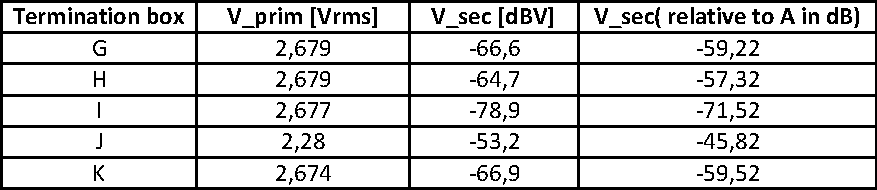
\includegraphics[width=0.9\textwidth]{img/task6_data.pdf} 
  \caption{Termination G-K observations}
  \label{fig:task6b} 
\end{figure}

\subsection{Is the inductive or capacitive noise that dominates for these terminations? Explain.}
From the observations it is seen that both the capacitive and inductive noises have been mostly eliminated with G-K,  except H which does not have shield and thus capacitive coupling dominates in this termination.  

\subsection{What is the biggest difference between the links in the C-F and G-K? Explain.}
In C-F, both the ends of shield are grounded providing a low impedance return path along ground which has larger loop area. In G-K only one end of the shield is grounded whereas the other end is shorted to the load, forcing the current return path along the shield which has much samller loop area. So G-K have much less inductive noise than G-K as observed above.

\subsection{Describe how the terminals G-K work and how the differences between them are involved.}
G: This termination is grounded at one end and the other end is connected to the load. As stated earlier grounding of shield reduces capacitative coupling. Since the other end of shield is connected to the load, the larger area ground return loop is removed, significantly eliminating induced inductive noise due to large area. Shield loop still exists but the shield is effectively close to the conductor and hence the loop area is much smaller. \\
H: In this termination with twisted pari, magnetic coupling is mostly reduced but since there is no shield, the electrical coupling is dominating and hence the attenuation is not much. \\
I: Here the twisted pair has a grounded shield and hence electrical coupling noise is reduced from H. But as the other end of shield is floating, shielding has no effect in further reducing magnetic field coupling. \\
J: In this shielding the shield is grounded at both ends which increases the area of low impedance ground loop and hence more magnetic noise is induced than others. \\
K: Since the other end of shield is connected to the load, the external ground loop is removed from J and hence inductive noise is reduced. \\

%% TASK 7
\section{This lab assignments largely follows an attempt made by Ott in the 70s.}
\subsection{Unlike Ott we have more turns on the coils. How will it affect measuring our performance compared to capacitive and inductive noise transmitted? Explain your answer.}
We know that if the number of turns of a coil increase, magnetic flux from the coil increases and hence its inductance. This means the magnetic coupling between two coils increases if we increase the number of turn of any coils. But the capacitive coupling remains unaffected by just increasing the number of turns.
\subsection{ The results Ott obtained were respectively: 0, 0, 27, 13, 13, 28, 80, 55, 70, 63 and 77 dB attenuation of link A-K, relative to the connector A. The values we measure will vary somewhat in relation to Ott. To what extent the values vary between the terminals? Compare the results you got with the Ott's ones. Do the results seem reasonable? Can you point out possible causes of the differences that you find? (is the tendency the same, or is there a discrepancy? Explain any discrepancies.)}
On comparing our lab data to that of Ott in textbook, we can say that out observation has higher noise. It can be explained by our coils having more turns than that of Ott. But the difference is not same for all terminations. Our best termination is I whereas Ott's is G. But Ott has explained that if twisted pair in termination I has large numbers of turns per uint length, then I could attenuate noise more than G. So out STP in I should have more number of turns than Ott's. \\
There can be other factors for our observations being different than that of Ott. Some of them may be the lab setup, instruments around the setup, oscilloscope setup (like sampling frequency), etc. However in general we can say that the trend of performance of various termination cards is similar with Ott.

%% TASK 8
\section{Measure the signal strength for type A-K at 20kHz, 500kHz and 2MHz. Record the results in a table and create a graphical representation of the development.}
Figure \ref{fig:task8} is the tabular presentation of input and output signal strength with A-K termination at 20 kHz, 500 kHz and 2 MHz. Similarly figure  \ref{fig:task8in} and  \ref{fig:task8out} shows the signal strength plots for input at the primary and output at the secondary coil  against frequency for all terminations.

\begin{figure} [H] %% table as picx
  \centering 
  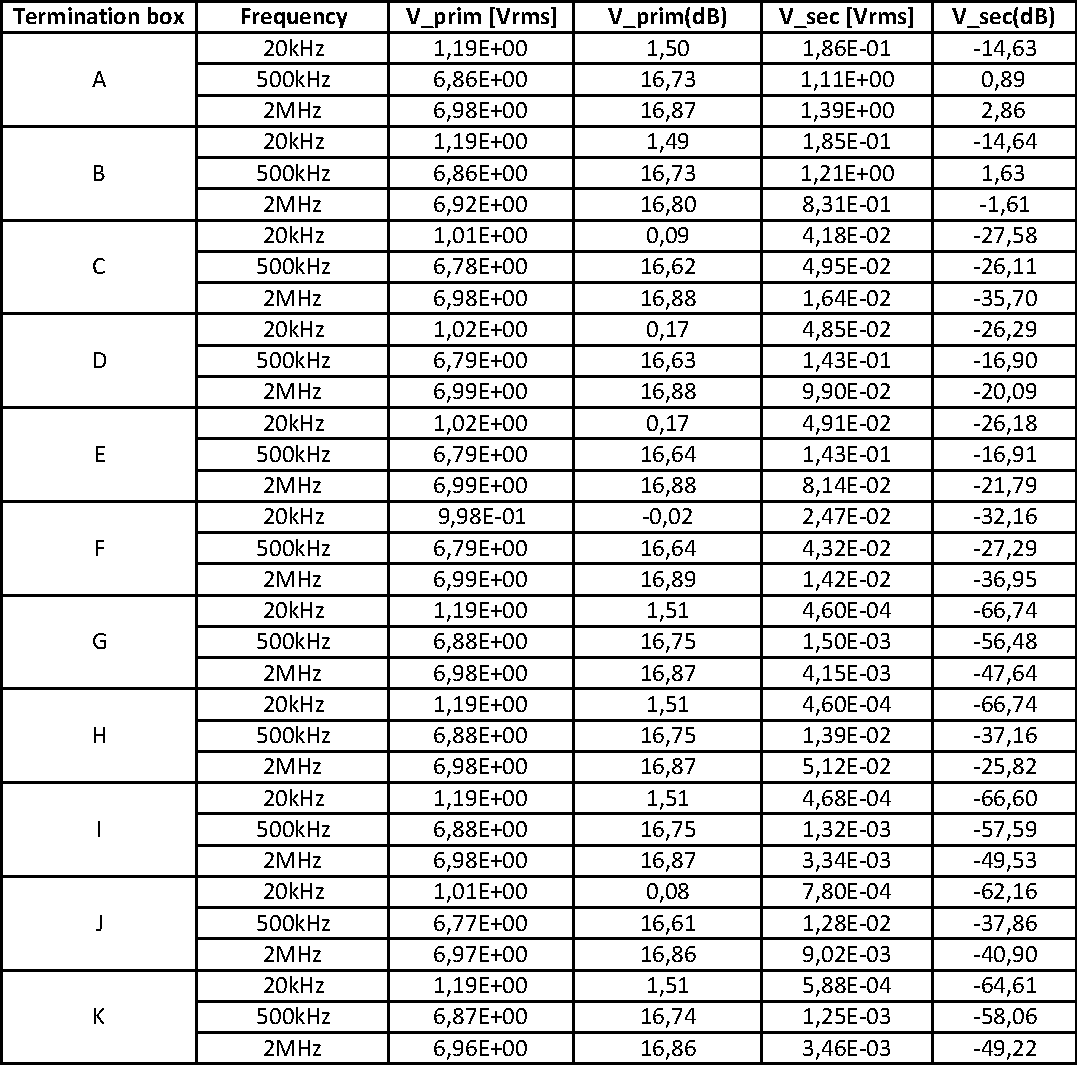
\includegraphics[width=1\textwidth]{img/task8_data.pdf} 
  \caption{Termination A-K observations at different frequency}
  \label{fig:task8} 
\end{figure}

\begin{figure} [H] %% table as picx
  \centering 
  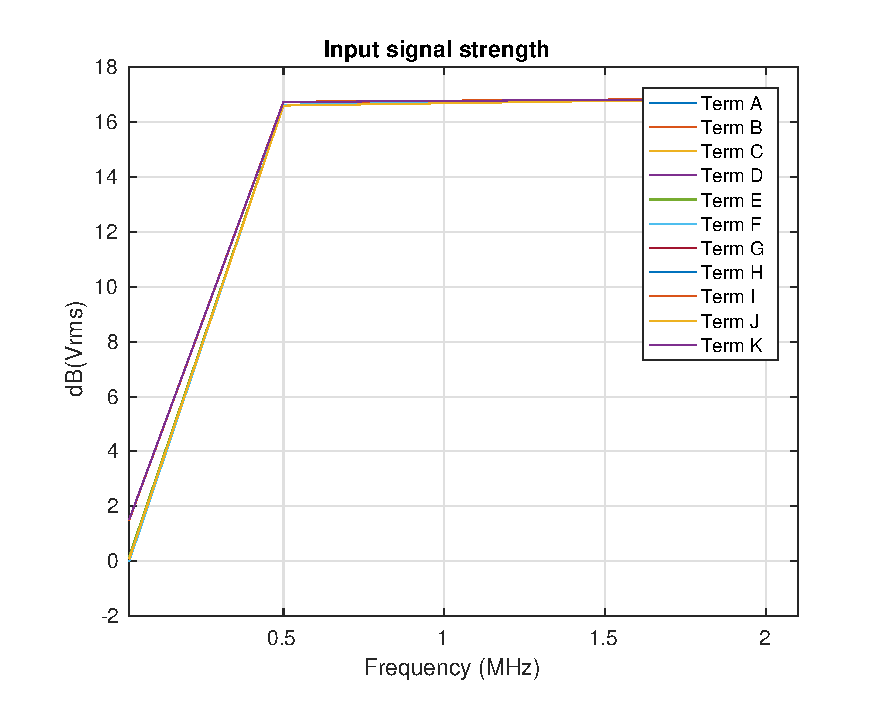
\includegraphics[width=0.85\textwidth]{img/input.eps} 
  \caption{Input strength with A-K terminations}
  \label{fig:task8in} 
\end{figure}

\begin{figure} [H] %% table as picx
  \centering 
  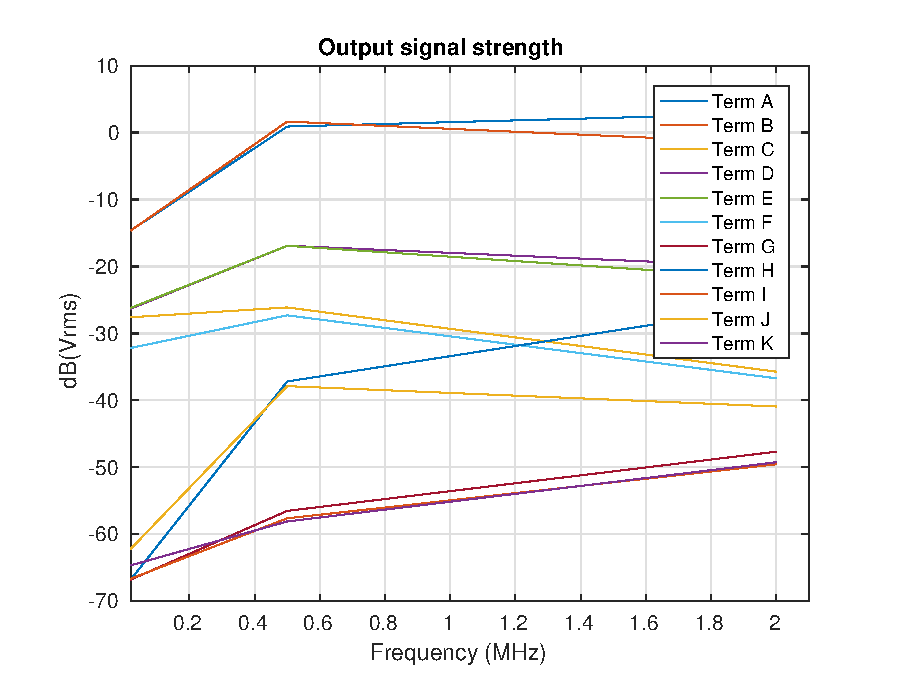
\includegraphics[width=0.85\textwidth]{img/output.eps} 
  \caption{Output strength with A-K terminations}
  \label{fig:task8out} 
\end{figure}

\subsection{How does the voltage of the function generator change for the different frequencies? (HINT: is the voltage source ideal or is there an internal resistance...?)} 
At low frequency the voltage of the function generator is much less because the internal resistance of signal source is much greater than the reactance of the conductor. At higher frequency the reactance of the conductor dominates and hence large voltage is dropped across the load.

\subsection{How does the ratio between inductive and capacitive noise change with frequency? Explain.}
At low frequency both capacitive and inductive noise are linearly proportional to frequency whereas at higher frequency both noises are independent of frequency. Hence the ratio is constant over frequency.

\subsection{Some of the terminals perform worse in comparison to the others at high frequencies, while some are apparently better. What could be the reason? (Comment the special relationship between H and J).}
We can comapare termination H and J performance in \ref{fig:task8out}. It is seen that J performs better at high frequency than H. Physically, H is TP only but J is STP which is like TP and coax together. At higher frequency due to skin effect, the noise current flows from the outer surface of the coax, thereby decreasing its effect on the signal current flowing on the core conductor. Hence J performs better at higher frequency than H.

\subsection{Compare these results with those from 50 kHz and those that Ott did. How and why do the characteristics of the various cables and termination types themselves change at higher frequencies?}
The parameters of conductor and shield like characteristic impedance and reactance are frequency dependent. In addition at higher frequency, effects like skin effect comes into play which changes current distrubution in the conductors. These factors change the characteristics of cables and terminations at higher frequencies.

%% TASK 9
\section{Measure the signal strength at 20, 50 and 500 kHz and 2MHz for termination A, C and G with the pure coax cable. Put these results in a table together with the results for STP cable from the task 5 and 8. (In addition to measurement data you should make a row / column where you normalise with respect to A for each cable at the current rate).}
\begin{figure} [H] %% table as picx
  \centering 
  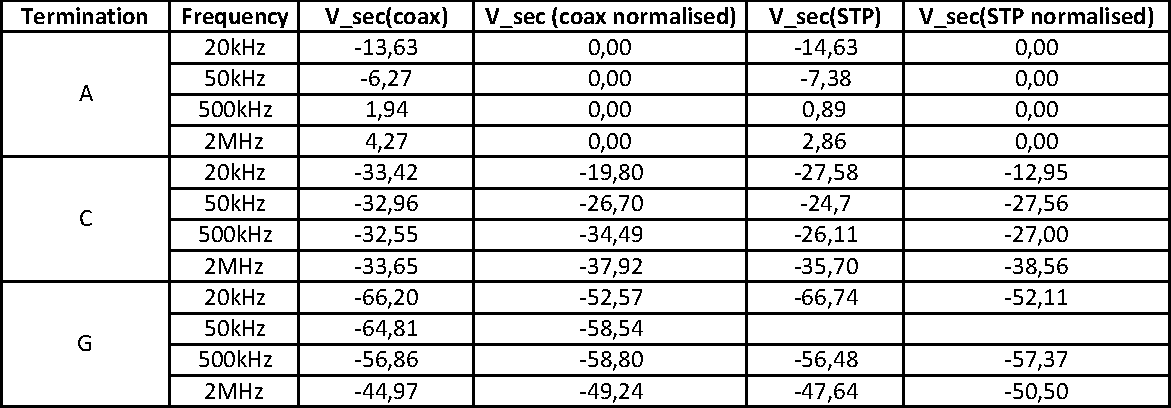
\includegraphics[width=0.9\textwidth]{img/task9_data.pdf} 
  \caption{Termination A, C and G with coax and STP}
  \label{fig:task9} 
\end{figure}

\subsection{Which of the links G / C tells us most about the impedance of the shield being high or low? Explain your answer.}
Termination G tells us about the impedance of the shield being high or low because in G the return current is forced to passed through the screen whereas in C the return current is passed through the ground plane.

\subsection{Which of the cables (pure coax vs STP) has the lowest impedance in the shield? Explain the basis of your results.}
In our results above the average signal strength in STP is less than that in coax. Hence it can be said that STP has the lowest impedance.

\subsection{In the data sheet for STP cable is given a lead to lead capacitance of 112pF / m and capacitance between wire to shield of 220pF / m, while Coax have a capacitance of 54pF / m between wire and shield. How well does this fit with the measured results? Explain.}
We know that larger the capacitance between shield and concducting wire, less is the capacitive coupling. From the data sheet, it is known that STP has larger capacitance between wire to shield than coax and from the above results, we can see that STP performs better than coax. Hence we can conclude that data sheet specification fits with our measured results. 

%%TASK 10
\section{Measure the signal strength at 20, 50 and 500 kHz and 2MHz for termination A, D and H twisted pair (TP) - and speaker (HTT) cables. Write down the results. Make a table where you normalize the results with respect to A for each frequency and cable.}
\begin{figure} [H] %% table as picx
  \centering 
  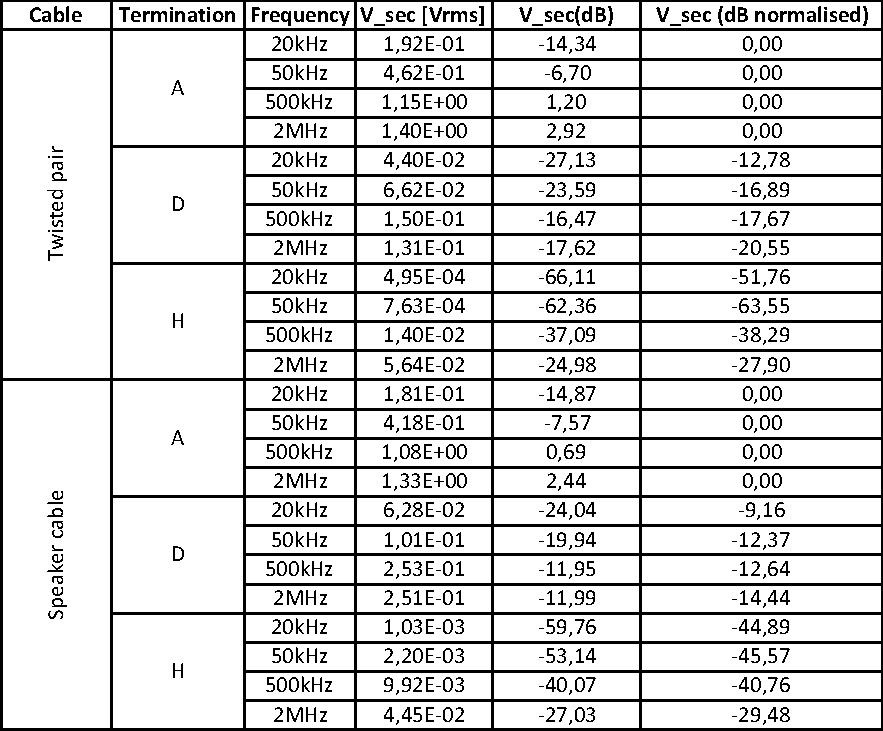
\includegraphics[width=0.8\textwidth]{img/task10_data.pdf} 
  \caption{Termination A, D and H with TP and HTT cables}
  \label{fig:task10} 
\end{figure}
\subsection{Should coupling D or H tell us most about the effect of twisting? (Explain your answer)}
Coupling H tells us most about the effect of twisting because in D the twisting effect is reduced by the large ground loop formed by grounding both ends.
\subsection{Have twisting any appreciable effect in this case, or are there other characteristics of cables that are more applicable here? Explain. (Hint: dielectric properties ...)}
Twisting does have appreciable effect as more twisting results in more reduction in magnetic coupling. Dielectric substance between the two conductors also affects the characteristic of twisted cable because substance with high dielectric constant creates more capacitance between the twisted pair wires.
%%TASK11 

\section{For cat5e cable, there are three pairs.}
\subsection{Can you rank the green (white sleeve  pair 3), orange (yellow sleeve pair 2) and brown (red sleeve  pair 4) wire pairs according to which has more twist per meter, only based on measurements of noise? Explain the termination card and frequency (s) you want and why you want to use these. Write down the results of the  measurements and explain your findings.}
We have chosen termination H and frequency 50 kHz and 500 kHz because in exercise 10.1, we concluded that H is better choice to observe the effect of twisting. Moreover at 50 kHz frequency, there was largest attenuation. 500kHz is taken to seen how the performance of wire differ in higher frequency. 

\begin{figure} [H] %% table as picx
  \centering 
  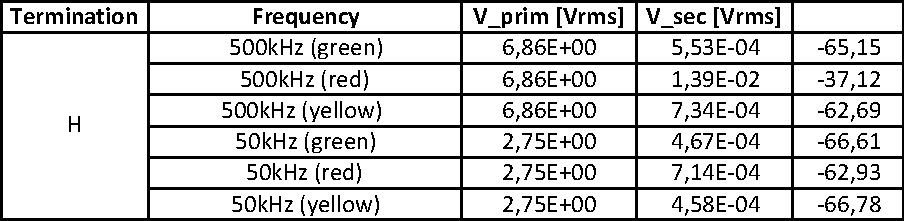
\includegraphics[width=0.8\textwidth]{img/task11a_data.pdf} 
  \caption{cat5e wires attenuation}
  \label{fig:task11a} 
\end{figure}
From the above results, we can see that green has more twists per meter on average and red/brown has less twists per meter.

\subsection{See "cat5e" in Wikipedia. Compare this result with your table "Individual twist lengths" from Wikipedia. Are the results in disagreement? Explain.}
Wikipedia states that green has 65, orange has 56 and brown has 52 twists per meter which is in agreement with our result above.
\subsection{The white sleeve contains both the green (pair 3) and blue (pair 1) pairs. Let's consider the shielding properties of the cables by using termination H and I. Measure the noise level using the two terminations for 20kHz, 50kHz, 500kHz, and 2MHz.}
\begin{figure} [H] %% table as picx
  \centering 
  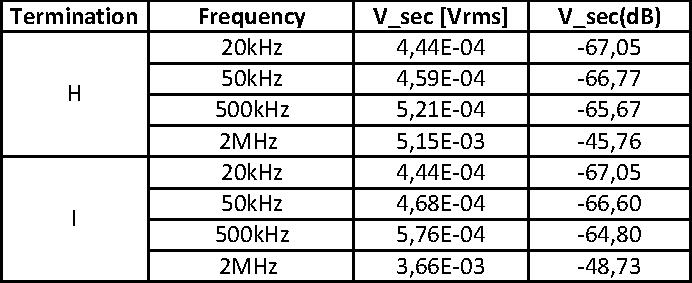
\includegraphics[width=0.6\textwidth]{img/task11c_data.pdf} 
  \caption{cat5e green/blue pairs with terminations H and I}
  \label{fig:task11c} 
\end{figure}
\subsubsection{Does the blue pair act as shield for the green pair? What shield effect can we see here?}
From the above result, it looks like the blue pair acts as shield for the green pair. Even though termination H is without shield, the above result for H is even better than I because the blue pair is shielding the green pair even when unshielded termination is applied.
\subsubsection{Compare this result with the difference between H and I in task 5 and 8. Explain any differences and similarities.}
On comparing our results from this task with that of task 5 and 8, we see that termination I has similar performance but termination H has much difference. In all the tasks stermination I is technically same, ie TP with shield and hence have similar result. But termination H in this task is equivalent to termination I as the blue pair is shielding the green pair and hence I here has better attenuation than in task 5 and 8.

\end{document}

